% Main LaTeX Document for Springer Nature LNCS Proceedings
% Modular Multi-Author Setup for 4-Member Team Project
% Course: Machine Learning - Project 5: Reinforcement Learning-Based Game Agent

\documentclass[runningheads]{llncs}

\usepackage[T1]{fontenc}
\usepackage{graphicx}
\usepackage{booktabs}
\usepackage{amsmath}
\usepackage{amssymb}
\usepackage{url}
\usepackage{cite}
\usepackage{tabularx}
\usepackage{subcaption}

\begin{document}

\title{Autonomous Navigation in 2D Platformers: A Curriculum-Driven Evaluation of Tabular Q-Learning and Hybrid Expected Q-SARSA}
\titlerunning{Evaluation of Tabular and Hybrid Q-SARSA in 2D Platformers}

\author{Member 1\inst{1} \and
Member 2\inst{1} \and
Member 3\inst{1} \and
Member 4\inst{1}\thanks{Corresponding evaluation author: responsible for empirical evaluation, statistical verification, and Section 7.}}

\authorrunning{Team Mario Agent et al.}

\institute{Department of Computer Science and Engineering\\
University Team Project --- Reinforcement Learning Course\\
\email{evaluation-member4@university.edu}}

\maketitle

% =========================================================================
% MODULAR SECTIONS (Each member edits their assigned section file)
% =========================================================================

% Abstract (Joint / Lead: Member 4)
\begin{abstract}
Autonomous navigation in dynamic platformer environments presents a classic reinforcement learning challenge characterized by delayed credit assignment and perceptual aliasing. This paper evaluates a tabular Q-learning agent deployed in a custom 2D graveyard platformer entitled \textit{Ho{\'a}'s Midnight Escape}, featuring a compact 144-state discretization space and a multi-stage curriculum progression. Training is governed by an asymmetric progress-shaped reward function balancing forward momentum and pit avoidance. While team members contributed environment physics, state discretization, and training orchestration, this paper focuses rigorously on empirical evaluation and statistical verification across 1,200 training episodes across three complexity tiers. The agent achieves a 99.0\% win rate on Level 1, 93.0\% on Level 2, and 88.0\% on Level 3 in the converged regime. Two-sample Welch's $t$-tests confirm statistically significant reward improvements from early exploration to convergence ($t = 23.41, 22.77, 22.90$ for Levels 1--3, all $p < 0.001$), accompanied by substantial reductions in navigation steps and collision rates. We present comprehensive learning curves, reward profiling benchmarks, playstyle clustering matrices, and failure mode decompositions demonstrating the efficacy of curriculum-based policy transfer in discrete state representations.

\keywords{Reinforcement Learning \and Tabular Q-Learning \and Curriculum Learning \and State Discretization \and Empirical Evaluation \and Statistical Hypothesis Testing.}
\end{abstract}


% Section 1: Introduction (Joint / Lead: Member 1 & Member 4)
\section{Introduction}
\label{sec:intro}

Reinforcement learning (RL) has emerged as a cornerstone of autonomous decision-making in sequential control tasks and interactive video games~\cite{mnih2015human,sutton2018reinforcement}. Classic 2D platformers represent a formidable testbed because they demand continuous temporal precision, rapid reaction to moving and stationary hazards, and robust spatial navigation. Unlike discrete grid-worlds, platformers feature continuous kinematic properties, requiring jump timing calibrated to gravitational acceleration, obstacle heights, and pit widths.

In this university team project, we design, implement, and evaluate an autonomous game agent navigating a 2D graveyard platformer entitled \textit{Ho{\'a}'s Midnight Escape}. In this scenario, the protagonist Ho{\'a} awakens in an eerie midnight graveyard and must navigate through tall tombstones, open burial pits, and airborne hazards to reach the safety of his home. Initially, the agent possesses no prior domain knowledge; through trial-and-error interaction and environmental feedback, it acquires an optimal control policy.

The primary motivation of this work is to demonstrate that an interpretable, resource-efficient Tabular Q-Learning agent can achieve high navigational proficiency in continuous 2D games when coupled with domain-specific spatial discretization and structured curriculum learning. To prevent merge friction and maintain software engineering rigor across our four-member team, our application decouples game physics, state representation, reward formulation, and empirical evaluation via explicit abstract interfaces.

The remainder of this paper is structured as follows: Section~\ref{sec:related} reviews related literature in game AI and reinforcement learning. Section~\ref{sec:objectives} outlines project objectives and technical gaps. Section~\ref{sec:teamwork} describes team task distribution, software workflow, and project management. Section~\ref{sec:approach} details the input/output representation, Q-learning algorithms, and modular reward strategies. Section~\ref{sec:impl} discusses system architecture, UI design, tech stack, and code highlights. Section~\ref{sec:eval} presents an extensive empirical evaluation with statistical significance tests across curriculum tiers. Finally, Section~\ref{sec:conclusion} concludes the paper with reflections and future research directions.


% Section 2: Related Work (Lead: Member 2 & Member 3)
\section{Related Work}
\label{sec:related}

Autonomous gameplay in 2D platformers has long served as a standard benchmark for artificial intelligence, spanning classical search, evolutionary computation, and reinforcement learning.

\subsection{Reinforcement Learning in Video Games}
Model-free Temporal Difference (TD) algorithms, initiated by Watkins~\cite{watkins1992q}, form the mathematical foundation for learning optimal policies without explicit transition probability models. The integration of deep neural networks with Q-learning (Deep Q-Networks, DQN) by Mnih et al.~\cite{mnih2015human} enabled agents to learn directly from raw video pixels in Atari 2600 environments. In the context of platformers like Nintendo's \textit{Super Mario Bros.}, deep reinforcement learning methods, including Proximal Policy Optimization (PPO)~\cite{schulman2017proximal} and Asynchronous Advantage Actor-Critic (A3C), have demonstrated impressive capabilities in navigating complex stages~\cite{khalid2024mario}. However, deep RL methods require millions of environment steps, specialized GPU hardware, and extensive hyperparameter tuning, frequently operating as black-box systems with high training instability.

\subsection{State Discretization and Tabular Control}
When computational resources or real-time constraints preclude deep neural architectures, state space quantization offers a compelling, interpretable alternative~\cite{sutton2018reinforcement}. By partitioning continuous spatial coordinates into discrete spatial bins, tabular methods maintain exact $Q(s, a)$ lookup tables with provable convergence guarantees. Early work by Sutton demonstrated that feature tile-coding and domain-specific bucketing can effectively mitigate the curse of dimensionality. Our work builds upon this principle by discarding global world coordinates in favor of invariant relative hazard distance features.

\subsection{Curriculum Learning and Reward Shaping}
Curriculum learning, introduced by Bengio et al.~\cite{bengio2009curriculum}, structures training by presenting task variants of increasing difficulty. In robotic locomotion and obstacle avoidance, curriculum schedules prevent agents from falling into local failure traps during early training~\cite{chen2024curriculum,ray2024dynamic}. In parallel, reward shaping—formalized by Ng et al. in potential-based reward theory—accelerates learning in sparse domains. Recent studies have demonstrated that asymmetric progress penalties effectively eradicate cyclical stalling and dithering behaviors in obstacle navigation benchmarks~\cite{zhang2023comparative}.


% Section 3: Objectives, Problem Description, and Research Gaps (Lead: Member 2 & Member 3)
\section{Objectives, Problem Description, and Research Gaps}
\label{sec:objectives}

\subsection{Problem Formulation (Markov Decision Process)}
We formulate the platformer navigation challenge as a discrete-time Markov Decision Process (MDP) defined by the 5-tuple $(\mathcal{S}, \mathcal{A}, \mathcal{P}, \mathcal{R}, \gamma)$:
\begin{itemize}
    \item \textbf{Environment}: A 2D side-scrolling platformer with continuous kinematic physics ($60\text{ FPS}$), featuring variable-height tombstones, lethal open chasms, dynamic airborne ghosts, warmth collectibles, and a terminal goal house.
    \item \textbf{Continuous State Space}: In raw game physics, the agent is governed by real-valued kinematics $\mathbf{s}_{\text{raw}} = (x, y, v_x, v_y) \in \mathbb{R}^4$, along with arbitrary obstacle and pit coordinates. Because this space is uncountably infinite ($|\mathcal{S}_{\text{raw}}| \to \infty$), exact table lookup is intractable.
    \item \textbf{Action Space ($\mathcal{A}$)}: Five discrete actions: $\text{STAY} (0)$, $\text{LEFT} (1)$, $\text{JUMP} (2)$, $\text{RIGHT} (3)$, and $\text{RIGHT\_JUMP} (4)$.
    \item \textbf{Transition Function ($\mathcal{P}$)}: Governed by the underlying game engine kinematics including gravitational acceleration ($g = 0.5\text{ px/tick}^2$), terminal velocity, and AABB collision resolution.
    \item \textbf{Reward Signal ($\mathcal{R}$)}: Environmental reinforcement scalar driving the agent toward the goal while avoiding hazards.
    \item \textbf{Discount Factor ($\gamma$)}: Set to $\gamma = 0.99$ to prioritize long-term survival and eventual goal attainment.
\end{itemize}

\subsection{Identified Research Gaps and Technical Challenges}
Current approaches to platformer reinforcement learning face four major limitations:
\begin{enumerate}
    \item \textbf{Compute Inefficiency of Deep RL}: Deep architectures (such as DQN or PPO) require millions of frames, specialized compute infrastructure, and extensive tuning. For resource-constrained academic setups or lightweight game agents, deep networks introduce unnecessary complexity and latency.
    \item \textbf{Spatial Overfitting in Naive Discretization}: Prior tabular methods frequently partition absolute global coordinates ($x, y$). This destroys generalization: an agent trained on Level 1 cannot navigate Level 2 because world coordinates do not match. A spatially invariant feature representation is essential.
    \item \textbf{The Credit Assignment and Dithering Bottleneck}: Purely sparse reward signals ($+100$ on victory, $-50$ on death) provide no gradient in intermediate states, causing agents to timeout randomly. Conversely, symmetric dense progress rewards ($+1.0$ forward, $-1.0$ backward) allow agents to oscillate back and forth without penalty, resulting in policy dithering.
    \item \textbf{Maximization Bias and Exploratory Jitter Near Hazards}: Off-policy Q-learning assumes optimal future greedy actions ($\max_{a'}$). In the presence of lethal cliffs and moving adversaries, stochastic exploratory actions during training lead to sudden deaths that off-policy updates fail to anticipate, requiring expectation-based on-policy TD targets (Expected SARSA).
\end{enumerate}

\subsection{Project Objectives}
To address these gaps, our team established four concrete engineering and research objectives:
\begin{enumerate}
    \item Design a compact, spatially invariant 7-tuple discretization model ($\le 1{,}152$ discrete states) that abstracts continuous kinematics into relative hazard proximities without perceptual aliasing.
    \item Implement a modular, asymmetric progression reward function that discourages backward regression and policy dithering.
    \item Validate that curriculum-based policy transfer across a 5-tier environment enables tabular reinforcement learning to master increasingly complex platforming stages, resolving hard exploration bottlenecks where training from scratch fails.
    \item Formulate and comparatively benchmark a unified Hybrid Q-SARSA framework against pure off-policy Q-learning, demonstrating how policy-expectation bootstrapping (Expected SARSA) mitigates maximization bias near dynamic adversaries and lethal chasms.
\end{enumerate}


% Section 4: Teamwork & Project Management (Lead: Member 1, 2, 3, 4)
\section{Teamwork \& Project Management}
\label{sec:teamwork}

This project was developed by a four-member university engineering team over a multi-week development cycle. This section outlines our task distribution, software engineering workflow, and initial conceptual ideation.

\subsection{Task Distribution and Member Contributions}
To ensure clear accountability and parallel productivity, responsibilities were partitioned strictly across subsystem boundaries:

\begin{itemize}
    \item \textbf{Member 1 (Environment \& Physics Lead)}: Responsible for the 2D Pygame game loop, jump and gravity physics modeling, axis-aligned bounding box (AABB) collision detection, and multi-tier tilemap layouts.
    \item \textbf{Member 2 (Agent \& State Discretization Lead)}: Designed the invariant continuous-to-discrete spatial feature projection, implemented the hashable $Q$-table data structures, Bellman TD updates, and deterministic random tie-breaking.
    \item \textbf{Member 3 (Reward \& Training Orchestration Lead)}: Formulated the pluggable reward strategies (Sparse, Dense, Balanced), orchestrated the multi-episode curriculum loop, implemented $\epsilon$-decay schedules, and handled policy serialization.
    \item \textbf{Member 4 (Evaluation \& Empirical Reporting Lead --- Author of Section~\ref{sec:eval})}: Designed the automated telemetry logging pipeline, computed Welch's $t$-tests and effect sizes, generated academic-grade vector visualizations (Figures~\ref{fig:curriculum_win_rate}--\ref{fig:sample_efficiency}), performed failure mode breakdowns, and authored the empirical evaluation report.
\end{itemize}

\subsection{Workflow, Version Control, and Software Engineering Practices}
To avoid code conflicts and ensure seamless module integration, the team adopted several modern software engineering practices:
\begin{itemize}
    \item \textbf{Version Control and Branching}: The codebase was hosted on a private GitHub repository. Each member worked in dedicated feature branches (\texttt{feature/env-physics}, \texttt{feature/discretizer}, \texttt{feature/training-loop}, \texttt{feature/evaluation-telemetry}). Pull requests required peer review and smoke-test verification before merging into \texttt{main}.
    \item \textbf{Decoupled SOLID Architecture}: Subsystems were decoupled via abstract base classes in \texttt{core/interfaces.py} (\texttt{BaseEnvironment}, \texttt{BaseDiscretizer}, \texttt{BaseRewardStrategy}, \texttt{BaseAgent}). This ensured the Open/Closed and Dependency Inversion principles: modifications to game physics or tilemaps did not require modifications to the agent's Q-table update logic.
    \item \textbf{Communication and Bug Tracking}: Weekly synchronous sprint meetings were supplemented with asynchronous Discord communication. Technical bugs and task milestones were tracked using GitHub Issues and GitHub Projects Kanban boards.
\end{itemize}

\subsection{Ideation and Concept Development}
During initial brainstorming, the team explored several benchmark concepts, including grid-world mazes, Flappy Bird clones, and endless runners. We selected a continuous 2D graveyard platformer entitled \textit{Ho{\'a}'s Midnight Escape} because it combined continuous jump kinematics with non-trivial hazard diversity (variable-height gravestones, chasms, and airborne obstacles). The narrative framing provided clear physical constraints that guided reward shaping and curriculum design.


% Section 5: Proposed Approach (Lead: Member 2 & Member 3)
\section{Proposed Approach}
\label{sec:approach}

This section details the theoretical and algorithmic formulation of our reinforcement learning system, authored collaboratively by Members 2 and 3.

\subsection{State Representation and Discretization Mapping}
To eliminate the curse of dimensionality and ensure spatial invariance across different level layouts, the continuous coordinate state $\mathbf{s}_{\text{raw}}$ is mapped into a compact, discrete 7-tuple:
\begin{equation}
\mathcal{S} = \langle \text{is\_grounded}, \; V_{y\text{-sign}}, \; \text{Obstacle}_{\text{dist}}, \; \text{Obstacle}_{\text{height}}, \; \text{Pit}_{\text{dist}}, \; \text{Ghost}_{\text{dist}}, \; \text{Ghost}_{\text{alt}} \rangle
\end{equation}

The individual feature dimensions are partitioned as follows:
\begin{enumerate}
    \item \textbf{Grounded Status ($\text{is\_grounded} \in \{0, 1\}$)}: Binary flag ($1$ if feet touch ground, $0$ otherwise), preventing illegal mid-air jumps.
    \item \textbf{Vertical Velocity Sign ($V_{y\text{-sign}} \in \{-1, 0, 1\}$)}: Distinguishes ascending jumps ($v_y < -0.1 \implies 1$), descending falls ($v_y > 0.1 \implies -1$), and horizontal motion ($0$).
    \item \textbf{Obstacle Proximity ($\text{Obstacle}_{\text{dist}} \in \{0, 1, 2, 3\}$)}: Measures distance to the nearest upcoming obstacle: $\text{NONE} (0, > 80\text{ px})$, $\text{FAR} (1, 45\text{--}80\text{ px})$, $\text{CLOSE} (2, 15\text{--}45\text{ px})$, and $\text{IMMEDIATE} (3, < 15\text{ px})$. Vertically cleared obstacles reset to $\text{NONE} (0)$.
    \item \textbf{Obstacle Height ($\text{Obstacle}_{\text{height}} \in \{0, 1\}$)}: Binary height threshold: $\text{LOW} (0, \le 50\text{ px})$ vs. $\text{HIGH} (1, > 50\text{ px})$.
    \item \textbf{Pit Proximity ($\text{Pit}_{\text{dist}} \in \{0, 1, 2\}$)}: Quantizes distance to lethal chasms into $\text{NONE} (0, > 100\text{ px})$, $\text{FAR} (1, 32\text{--}100\text{ px})$, and $\text{IMMEDIATE} (2, \le 32\text{ px})$, defining the safe take-off zone.
    \item \textbf{Ghost Proximity ($\text{Ghost}_{\text{dist}} \in \{0, 1, 2, 3\}$)}: Measures horizontal distance to moving ghosts: $\text{NONE} (0, > 80\text{ px})$, $\text{FAR} (1, 35\text{--}80\text{ px})$, $\text{CLOSE} (2, 0 < \text{dist} \le 35\text{ px})$, and $\text{OVERLAP} (3, \text{dist} = 0\text{ px})$.
    \item \textbf{Ghost Altitude ($\text{Ghost}_{\text{alt}} \in \{0, 1\}$)}: Indicates whether a ghost flies low ($\text{LOW} = 0$, requiring a jump over) or high ($\text{HIGH} = 1$, allowing walking underneath).
\end{enumerate}

The resulting combinatorial cardinality of this quantized state space is:
\begin{equation}
|\mathcal{S}| = 2 \times 3 \times 4 \times 2 \times 3 \times 4 \times 2 = 1{,}152 \text{ discrete states.}
\end{equation}
In baseline levels without dynamic adversaries (Levels 1--3), ghost bins remain at zero, collapsing the effective state space to $144$ states. In adversary levels (Levels 4--5), the state space expands up to $1{,}152$ states. Even at maximum capacity, this compact representation allows rapid tabular value convergence without neural function approximation.

\subsection{Tabular Q-Learning Algorithm and Tie-Breaking}
The agent maintains an explicit lookup table $Q: \mathcal{S} \times \mathcal{A} \to \mathbb{R}$. During interaction, actions are selected using an $\epsilon$-greedy policy with deterministic random tie-breaking. At initialization ($Q(s, a) = 0$), standard \texttt{argmax} introduces severe index-0 bias (\texttt{STAY}); our agent instead identifies all maximal candidates $\mathcal{A}^* = \{a \in \mathcal{A} \mid Q(s, a) = \max_{a'} Q(s, a')\}$ and samples uniformly:
\begin{equation}
a_t = \begin{cases}
\text{Uniform}(\mathcal{A}), & \text{with probability } \epsilon \\
\text{Uniform}(\mathcal{A}^*), & \text{with probability } 1 - \epsilon
\end{cases}
\end{equation}

Upon executing $a_t$, transitioning to $s_{t+1}$, and receiving scalar reward $r_{t+1}$, the Q-value is updated via the off-policy Temporal Difference (TD) rule~\cite{watkins1992q}:
\begin{equation}
Q(s_t, a_t) \leftarrow Q(s_t, a_t) + \alpha \left[ r_{t+1} + \gamma \max_{a' \in \mathcal{A}} Q(s_{t+1}, a') - Q(s_t, a_t) \right]
\end{equation}
with learning rate decaying linearly from $\alpha_{\text{start}} = 0.12$ down to $\alpha_{\min} = 0.02$, and discount factor $\gamma = 0.99$. Exploration decays after each episode according to $\epsilon_{k+1} = \max(\epsilon_{\min}, \epsilon_k \cdot \lambda_{\text{decay}})$.

\subsection{Hybrid Q-SARSA Framework: Unifying On-Policy and Off-Policy Control}
\label{subsec:hybrid_formulation}
While pure Q-learning optimizes the optimal action-value function $Q^*$ by assuming greedy exploitation at future steps, it suffers from maximization bias and high risk near lethal hazards under exploratory jitter~\cite{sutton2018reinforcement}. On-policy SARSA, conversely, incorporates exploratory actions into its target, resulting in cautious policies that may freeze or fail to commit near cliffs. To overcome this dilemma, we architect a unified \textbf{Hybrid Q-SARSA Agent} supporting three target calculation paradigms~\cite{van2009theoretical,de2018multi}:

\paragraph{1. Expected SARSA Mode.}
Expected SARSA eliminates the sampling variance of classic SARSA while directly accounting for the stochastic exploratory behavior policy $\pi$ in the bootstrap target:
\begin{equation}
\label{eq:expected_sarsa}
\mathcal{T}_{\text{Expected}} = r_{t+1} + \gamma \sum_{a' \in \mathcal{A}} \pi(a' \mid s_{t+1}) Q(s_{t+1}, a')
\end{equation}
Under our $\epsilon$-greedy exploratory policy with uniform random tie-breaking over greedy candidates $\mathcal{A}^*$, the expected future return expands to:
\begin{equation}
\mathcal{T}_{\text{Expected}} = r_{t+1} + \gamma \left[ (1 - \epsilon) \max_{a' \in \mathcal{A}} Q(s_{t+1}, a') + \frac{\epsilon}{|\mathcal{A}|} \sum_{a' \in \mathcal{A}} Q(s_{t+1}, a') \right]
\end{equation}
During evaluation ($\epsilon = 0$), $\mathcal{T}_{\text{Expected}}$ smoothly reduces to the deterministic greedy Bellman target. During training ($\epsilon > 0$), the second term explicitly penalizes boundary states where an unintended exploratory action would plunge the agent into a lethal pit or adversary.

\paragraph{2. Linear $Q(\sigma)$ Target Interpolation.}
To explore the continuous spectrum between on-policy SARSA and off-policy Q-learning, we implement the $Q(\sigma)$ interpolation target~\cite{de2018multi} parameterized by mixing parameter $\beta \in [0, 1]$:
\begin{equation}
\label{eq:linear_q_sarsa}
\mathcal{T}_{\text{Linear}} = r_{t+1} + \gamma \left[ \beta Q(s_{t+1}, a_{t+1}) + (1 - \beta) \max_{a' \in \mathcal{A}} Q(s_{t+1}, a') \right]
\end{equation}
Setting $\beta = 0.0$ recovers pure Q-learning, $\beta = 1.0$ recovers on-policy SARSA, and $\beta = 0.25$ provides an empirically tuned compromise between greedy pursuit and trajectory-grounded safety.

\paragraph{3. Hazard-Gated Hybrid Mode.}
To address the physical asymmetry of platformer navigation---where open corridors reward fast momentum while chasm edges require precise commitment---our agent implements state-conditioned hazard gating:
\begin{equation}
\label{eq:hazard_gated}
\mathcal{T}_{\text{Gated}} = \begin{cases}
r_{t+1} + \gamma \max_{a' \in \mathcal{A}} Q(s_{t+1}, a'), & \text{if } \text{Pit}_{\text{dist}} \ge 1 \lor \text{Ghost}_{\text{dist}} \ge 1 \\
r_{t+1} + \gamma \left[ \beta Q(s_{t+1}, a_{t+1}) + (1 - \beta) \max_{a' \in \mathcal{A}} Q(s_{t+1}, a') \right], & \text{otherwise (safe corridor)}
\end{cases}
\end{equation}
In the proximity of lethal hazards, pure off-policy Q-learning eliminates hesitation and cliff-freezing by optimizing the ideal leap trajectory; along safe corridors, on-policy blending curbs reckless sprinting and reduces collision fatalities. In all variants, the TD update rule takes the unified form:
\begin{equation}
Q(s_t, a_t) \leftarrow Q(s_t, a_t) + \alpha \left[ \mathcal{T}_{\text{mode}} - Q(s_t, a_t) \right]
\end{equation}

\subsection{Curriculum Transfer and Continual Rehearsal}
In our curriculum framework, rather than training an agent on each stage from scratch, the learned Q-table is carried forward across progressive stages. When advancing to subsequent levels, the exploration rate re-warms to $\epsilon_0 = 0.30$ on Levels 2--3 and $\epsilon_0 = 0.40$ on Levels 4--5. This provides sufficient exploration to discover solutions for novel obstacles while retaining core locomotion skills.

To prevent catastrophic forgetting when training on complex stages (Levels 3--5), we employ an experience replay rehearsal mechanism~\cite{rolnick2019experience,isele2018selective}. Specifically, a replay ratio of $\rho = 0.35$ executes periodic updates over earlier level transitions. This allows the Q-table to master the current level's hazards without overwriting foundational jumping reflexes from prior stages~\cite{narvekar2020curriculum}.

\subsection{Modular Reward Shaping Formulations}
To prevent reward hacking and cyclical dithering, our primary production strategy (\texttt{BalancedRewardStrategy}) employs asymmetric horizontal progress shaping:
\begin{equation}
r_{t+1} = r_{\text{progress}}(\Delta x) + r_{\text{goal}} \cdot \mathbb{I}_{\text{win}} + r_{\text{pit}} \cdot \mathbb{I}_{\text{pit}} + r_{\text{ghost}} \cdot \mathbb{I}_{\text{ghost}} + r_{\text{item}} \cdot \mathbb{I}_{\text{item}} + r_{\text{obstacle}} \cdot \mathbb{I}_{\text{hit}} + r_{\text{step}}
\end{equation}
where:
\begin{equation}
r_{\text{progress}}(\Delta x) = \begin{cases}
+1.0 \cdot \Delta x, & \text{if } \Delta x > 0 \quad (\text{forward motion}) \\
-1.5 \cdot |\Delta x|, & \text{if } \Delta x \le 0 \quad (\text{backward regression})
\end{cases}
\end{equation}
with terminal victory bonus $r_{\text{goal}} = +200.0$, pit and ghost death penalties $r_{\text{pit}} = r_{\text{ghost}} = -75.0$, collectible warmth bonus $r_{\text{item}} = +30.0$, obstacle collision penalty $r_{\text{obstacle}} = -3.0$, and per-step living cost $r_{\text{step}} = -0.1$. The $1.5\times$ penalty on retreat ensures that oscillating backward is mathematically unprofitable, eliminating dithering.


% Section 6: Implementation Details (Lead: Member 1, Member 2, Member 3)
\section{Implementation Details}
\label{sec:impl}

This section describes the software architecture, graphical user interface, technology stack, and critical code highlights, authored collaboratively by Members 1, 2, and 3.

\subsection{Software Architecture and Decoupled Subsystems}
The project follows a decoupled, object-oriented design adhering to SOLID principles. The system is partitioned into five distinct Python packages under \texttt{core/interfaces.py}:
\begin{enumerate}
    \item \texttt{env/}: Houses the Pygame environment, continuous physics simulation, collision engine, and procedural tilemap loaders for Levels 1--5.
    \item \texttt{discretizer/}: Implements \texttt{BaseDiscretizer}, encapsulating continuous coordinate projection into the discrete 7-tuple hashable representation ($\le 1{,}152$ states).
    \item \texttt{rewards/}: Implements the Strategy Pattern via \texttt{BaseRewardStrategy}, allowing plug-and-play swapping between Sparse, Dense, and Balanced reward formulations without touching environment physics.
    \item \texttt{agent/}: Implements \texttt{BaseAgent}, providing both \texttt{TabularQAgent} (pure off-policy Q-learning) and \texttt{HybridQSARSAAgent} (Expected SARSA, linear $Q(\sigma)$ blending, and hazard-gated switching), alongside experience rehearsal, Q-table serialization, and decay schedulers.
    \item \texttt{evaluation/}: Houses telemetry loggers, CSV export hooks, and automated Matplotlib/Seaborn graph generation scripts.
\end{enumerate}

\subsection{User Interface and Interactive Modes}
The application provides two execution modes:
\begin{itemize}
    \item \textbf{Interactive GUI / Evaluation Mode}: Renders at $60\text{ FPS}$ using Pygame. The head-up display (HUD) visualizes real-time metrics, including current episode index, instantaneous reward, exploration rate $\epsilon$, current discrete state tuple $\langle s_1, \dots, s_7 \rangle$, and selected action. A manual keyboard mode (\texttt{play\_human.py}) allows human benchmark play.
    \item \textbf{Headless Training Mode}: Bypasses graphical rendering to execute physics steps at over $500\text{ FPS}$, accelerating multi-episode curriculum completion.
\end{itemize}

\subsection{Tech Stack}
The system is implemented in Python 3.10 and relies on standard open-source libraries:
\begin{itemize}
    \item \textbf{Pygame 2.5}: Manages 2D sprite rendering, window events, delta-time clocks, and collision bounding boxes.
    \item \textbf{NumPy 1.26}: Handles matrix operations, Q-table indexing, candidate tie-breaking, and numerical array processing.
    \item \textbf{Pandas 2.2}: Manages tabular telemetry logging, data frame transformations, and rolling performance window calculations.
    \item \textbf{Matplotlib 3.8 \& Seaborn 0.13}: Renders publication-grade vector graphics (PDF) adhering to IEEE/Springer typographical styles.
\end{itemize}

\subsection{Code Highlights}
Listing~\ref{lst:tie_break} illustrates the deterministic uniform tie-breaking implementation in \texttt{agent/tabular\_q\_agent.py}, which eliminates early-stage action selection bias.

\begin{figure}[h]
\begin{center}
\begin{minipage}{0.9\textwidth}
\begin{verbatim}
def select_action(self, state: Tuple[int, ...]) -> int:
    if self.training and np.random.rand() < self.epsilon:
        return int(np.random.choice(self.num_actions))
    
    q_values = self.q_table[state]
    max_val = np.max(q_values)
    candidates = np.flatnonzero(q_values == max_val)
    return int(np.random.choice(candidates))
\end{verbatim}
\end{minipage}
\end{center}
\caption{Deterministic random tie-breaking during action selection.}
\label{lst:tie_break}
\end{figure}


% Section 7: Experimental Results & Evaluation (Lead: Member 4 [USER])
\section{Experimental Results \& Evaluation}
\label{sec:eval}

This section reports the test results for our agents across Levels~1--7. We compare two learning algorithms, two training modes, and three reward settings, and then look at sample efficiency, failure causes, and how well the saved agents work on new maps.

\subsection{Setup}
\label{subsec:setup}

We run all experiments on Levels~1--7 of \textit{Ho{\'a}'s Midnight Escape}. (The training script ran Levels~1--8 sequentially, and this evaluation focuses on the 7 core levels.) Each level runs for $10{,}000$ episodes, giving $70{,}000$ episodes across Levels~1--7. Every setting is repeated with $8$ independent random seeds ($42$ to $49$), which control both the agent and the environment.

We compare two agents: \textbf{Tabular Q-Learning} (which updates with the max next Q-value) and \textbf{Hybrid Expected SARSA} (which weights the next Q-values by the $\epsilon$-greedy policy). Both agents are tested in two training modes:
\begin{itemize}
    \item \textbf{Curriculum}: One Q-table starts on Level~1 and keeps training from Level~1 through Level~7. When entering a new level, exploration $\epsilon$ re-warms to at least $0.30$ on Levels~2--3 and $0.35$ on Levels~4--7. To reduce forgetting, after Level~1 the trainer also runs background replay episodes on earlier levels in round-robin order (configured with \texttt{replay\_ratio} $= 0.35$, implemented in \texttt{training/trainer.py} as a $\max(0.35, 0.5) = 0.50$ chance per episode of one greedy replay on a prior level, alongside replay of up to 5 stored winning paths).
    \item \textbf{Separate}: A fresh Q-table starts from scratch on each level with $\epsilon = 1.0$, without carry-over or prior-level replay.
\end{itemize}

We also test three reward functions: \textbf{Balanced} (our main shaped reward with forward/backward progress, item bonuses, hazard-timing guidance, and strong death/timeout penalties), \textbf{Dense} (goal-distance progress shaping with weaker penalties and no hazard-timing terms), and \textbf{Sparse} (only terminal goal/death signals and item bonuses).

For Levels~4--7, \texttt{training/trainer.py} uses a reverse-spawn schedule so the agent first practices closer to the goal and then moves back toward the start. In Curriculum mode, spawns step backward through fractions $(0.80, 0.60, 0.40, 0.20)$ of the goal distance before reaching the normal start, advancing when the agent passes a greedy check every 25 episodes or hits $1{,}428$ episodes in a segment (with $\epsilon$ reset to $0.30$ or $0.25$ and decay $0.985$ during reverse segments). In Separate mode, spawns follow fixed blocks of the $10{,}000$ episodes: $0.75$ of goal distance for episodes $1$--$1{,}800$ ($1.8\text{k}$), $0.50$ for $1{,}801$--$3{,}600$ ($3.6\text{k}$), $0.25$ for $3{,}601$--$5{,}400$ ($5.4\text{k}$), and the normal start for $5{,}401$--$10{,}000$, without re-warming $\epsilon$ between blocks. Table~\ref{tab:hyperparams} lists the shared training settings.

\begin{table}[t]
\caption{Main training hyperparameters used across Levels~1--7 (8 seeds: 42--49).}
\label{tab:hyperparams}
\centering
\begin{tabular}{ll}
\toprule
\textbf{Setting} & \textbf{Value} \\
\midrule
Episodes per level & $10{,}000$ ($70{,}000$ for Levels~1--7) \\
Learning rate ($\alpha$) & Linear decay $0.10 \to 0.005$ per level \\
Discount factor ($\gamma$) & $0.99$ \\
Exploration ($\epsilon$) & $1.0 \to 0.01$, decay $0.999$ per episode \\
Curriculum re-warm $\epsilon$ & $0.30$ (Levels~2--3), $0.35$ (Levels~4--7) \\
Replay ratio & $0.35$ (effective $0.50$ greedy prior-level replay) \\
Action repeat & $1$ \\
\bottomrule
\end{tabular}
\end{table}

To avoid mixing metrics, we define our four evaluation numbers clearly:
\begin{enumerate}
    \item \textbf{Train100}: Mean win rate over the last $100$ training episodes of a level (episodes $9{,}901$--$10{,}000$), averaged across the $8$ seeds (mean $\pm$ SD). Exploration is near $\epsilon = 0.01$ here.
    \item \textbf{Greedy50}: Mean win rate over $50$ pure greedy episodes ($\epsilon = 0.0$) run right after each level ends, averaged across the $8$ seeds.
    \item \textbf{All-10k Training Outcomes} (Section~\ref{subsec:failures}): Outcome shares (win, timeout, pit death, and hazard/entity death) averaged across all $10{,}000$ training episodes of a level.
    \item \textbf{1,000-Episode Procedural Test} (Section~\ref{subsec:checkpoint_eval}): Blind greedy evaluation ($\epsilon = 0.0$) of each saved best per-level checkpoint across $1{,}000$ newly generated procedural maps per level.
\end{enumerate}

\subsection{Overall Results \& Reward Choice}
\label{subsec:overall_rewards}

Table~\ref{tab:overall_winrates} gives the full scoreboard across all 7 levels, 2 agents, 2 training modes, and 3 rewards, and Fig.~\ref{fig:reward_trajectories} plots the smoothed episode returns over training.

\begin{table}[t]
\caption{Final Train100 and Greedy50 win rates (mean $\pm$ SD across 8 seeds) for Levels~1--7. $\Delta$ equals Hybrid minus Tabular on Train100.}
\label{tab:overall_winrates}
\centering
\resizebox{\textwidth}{!}{%
\begin{tabular}{llcccccc}
\toprule
\textbf{Level} & \textbf{Reward} & \textbf{Tabular Curr} & \textbf{Hybrid Curr} & \textbf{$\Delta$ Curr} & \textbf{Tabular Sep} & \textbf{Hybrid Sep} & \textbf{$\Delta$ Sep} \\
 & & \textbf{(Train100 / Greedy50)} & \textbf{(Train100 / Greedy50)} & \textbf{(Train100)} & \textbf{(Train100 / Greedy50)} & \textbf{(Train100 / Greedy50)} & \textbf{(Train100)} \\
\midrule
Level 1 & Balanced & 100.0 $\pm$ 0.0\% / 100.0 $\pm$ 0.0\% & 100.0 $\pm$ 0.0\% / 100.0 $\pm$ 0.0\% & +0.0\% & 100.0 $\pm$ 0.0\% / 100.0 $\pm$ 0.0\% & 100.0 $\pm$ 0.0\% / 100.0 $\pm$ 0.0\% & +0.0\% \\
Level 1 & Dense & 100.0 $\pm$ 0.0\% / 87.5 $\pm$ 35.4\% & 100.0 $\pm$ 0.0\% / 100.0 $\pm$ 0.0\% & +0.0\% & 100.0 $\pm$ 0.0\% / 100.0 $\pm$ 0.0\% & 100.0 $\pm$ 0.0\% / 100.0 $\pm$ 0.0\% & +0.0\% \\
Level 1 & Sparse & 99.0 $\pm$ 2.1\% / 62.5 $\pm$ 51.8\% & 87.5 $\pm$ 19.5\% / 50.0 $\pm$ 53.5\% & -11.5\% & 99.2 $\pm$ 2.1\% / 87.5 $\pm$ 35.4\% & 100.0 $\pm$ 0.0\% / 100.0 $\pm$ 0.0\% & +0.8\% \\
\midrule
Level 2 & Balanced & 90.8 $\pm$ 5.5\% / 100.0 $\pm$ 0.0\% & 60.6 $\pm$ 41.7\% / 62.5 $\pm$ 51.8\% & -30.1\% & 82.1 $\pm$ 26.9\% / 75.0 $\pm$ 46.3\% & 95.4 $\pm$ 5.4\% / 100.0 $\pm$ 0.0\% & +13.2\% \\
Level 2 & Dense & 41.8 $\pm$ 36.4\% / 53.8 $\pm$ 50.4\% & 55.0 $\pm$ 41.8\% / 50.0 $\pm$ 53.5\% & +13.2\% & 86.5 $\pm$ 9.3\% / 100.0 $\pm$ 0.0\% & 59.9 $\pm$ 42.4\% / 62.5 $\pm$ 51.8\% & -26.6\% \\
Level 2 & Sparse & 0.0 $\pm$ 0.0\% / 0.0 $\pm$ 0.0\% & 0.0 $\pm$ 0.0\% / 0.0 $\pm$ 0.0\% & +0.0\% & 0.0 $\pm$ 0.0\% / 0.0 $\pm$ 0.0\% & 0.0 $\pm$ 0.0\% / 0.0 $\pm$ 0.0\% & +0.0\% \\
\midrule
Level 3 & Balanced & 69.6 $\pm$ 30.1\% / 75.0 $\pm$ 46.3\% & 26.0 $\pm$ 32.9\% / 25.0 $\pm$ 46.3\% & -43.6\% & 80.5 $\pm$ 7.5\% / 100.0 $\pm$ 0.0\% & 67.6 $\pm$ 27.4\% / 87.5 $\pm$ 35.4\% & -12.9\% \\
Level 3 & Dense & 14.6 $\pm$ 30.9\% / 12.5 $\pm$ 35.4\% & 0.0 $\pm$ 0.0\% / 0.0 $\pm$ 0.0\% & -14.6\% & 16.5 $\pm$ 25.4\% / 25.0 $\pm$ 46.3\% & 60.8 $\pm$ 34.9\% / 75.0 $\pm$ 46.3\% & +44.2\% \\
Level 3 & Sparse & 0.0 $\pm$ 0.0\% / 0.0 $\pm$ 0.0\% & 0.0 $\pm$ 0.0\% / 0.0 $\pm$ 0.0\% & +0.0\% & 0.0 $\pm$ 0.0\% / 0.0 $\pm$ 0.0\% & 0.0 $\pm$ 0.0\% / 0.0 $\pm$ 0.0\% & +0.0\% \\
\midrule
Level 4 & Balanced & 0.0 $\pm$ 0.0\% / 0.0 $\pm$ 0.0\% & 0.0 $\pm$ 0.0\% / 0.0 $\pm$ 0.0\% & +0.0\% & 2.9 $\pm$ 8.1\% / 12.5 $\pm$ 35.4\% & 19.6 $\pm$ 19.0\% / 37.5 $\pm$ 51.8\% & +16.8\% \\
Level 4 & Dense & 0.0 $\pm$ 0.0\% / 0.0 $\pm$ 0.0\% & 0.0 $\pm$ 0.0\% / 0.0 $\pm$ 0.0\% & +0.0\% & 0.0 $\pm$ 0.0\% / 0.0 $\pm$ 0.0\% & 0.0 $\pm$ 0.0\% / 0.0 $\pm$ 0.0\% & +0.0\% \\
Level 4 & Sparse & 0.0 $\pm$ 0.0\% / 0.0 $\pm$ 0.0\% & 0.0 $\pm$ 0.0\% / 0.0 $\pm$ 0.0\% & +0.0\% & 0.0 $\pm$ 0.0\% / 0.0 $\pm$ 0.0\% & 0.0 $\pm$ 0.0\% / 0.0 $\pm$ 0.0\% & +0.0\% \\
\midrule
Level 5 & Balanced & 0.0 $\pm$ 0.0\% / 0.0 $\pm$ 0.0\% & 0.0 $\pm$ 0.0\% / 0.0 $\pm$ 0.0\% & +0.0\% & 0.0 $\pm$ 0.0\% / 0.0 $\pm$ 0.0\% & 0.0 $\pm$ 0.0\% / 0.0 $\pm$ 0.0\% & +0.0\% \\
Level 5 & Dense & 0.0 $\pm$ 0.0\% / 0.0 $\pm$ 0.0\% & 0.0 $\pm$ 0.0\% / 0.0 $\pm$ 0.0\% & +0.0\% & 0.0 $\pm$ 0.0\% / 0.0 $\pm$ 0.0\% & 0.0 $\pm$ 0.0\% / 0.0 $\pm$ 0.0\% & +0.0\% \\
Level 5 & Sparse & 0.0 $\pm$ 0.0\% / 0.0 $\pm$ 0.0\% & 0.0 $\pm$ 0.0\% / 0.0 $\pm$ 0.0\% & +0.0\% & 0.0 $\pm$ 0.0\% / 0.0 $\pm$ 0.0\% & 0.0 $\pm$ 0.0\% / 0.0 $\pm$ 0.0\% & +0.0\% \\
\midrule
Level 6 & Balanced & 21.2 $\pm$ 27.0\% / 25.0 $\pm$ 46.3\% & 7.8 $\pm$ 21.9\% / 12.5 $\pm$ 35.4\% & -13.5\% & 30.8 $\pm$ 27.9\% / 50.0 $\pm$ 53.5\% & 11.2 $\pm$ 15.7\% / 12.5 $\pm$ 35.4\% & -19.5\% \\
Level 6 & Dense & 0.2 $\pm$ 0.5\% / 0.0 $\pm$ 0.0\% & 0.8 $\pm$ 1.8\% / 0.0 $\pm$ 0.0\% & +0.5\% & 1.5 $\pm$ 4.2\% / 0.0 $\pm$ 0.0\% & 0.9 $\pm$ 2.5\% / 0.0 $\pm$ 0.0\% & -0.6\% \\
Level 6 & Sparse & 0.0 $\pm$ 0.0\% / 0.0 $\pm$ 0.0\% & 0.0 $\pm$ 0.0\% / 0.0 $\pm$ 0.0\% & +0.0\% & 0.0 $\pm$ 0.0\% / 0.0 $\pm$ 0.0\% & 0.0 $\pm$ 0.0\% / 0.0 $\pm$ 0.0\% & +0.0\% \\
\midrule
Level 7 & Balanced & 0.0 $\pm$ 0.0\% / 0.0 $\pm$ 0.0\% & 0.0 $\pm$ 0.0\% / 0.0 $\pm$ 0.0\% & +0.0\% & 0.0 $\pm$ 0.0\% / 0.0 $\pm$ 0.0\% & 0.0 $\pm$ 0.0\% / 0.0 $\pm$ 0.0\% & +0.0\% \\
Level 7 & Dense & 0.0 $\pm$ 0.0\% / 0.0 $\pm$ 0.0\% & 0.0 $\pm$ 0.0\% / 0.0 $\pm$ 0.0\% & +0.0\% & 0.0 $\pm$ 0.0\% / 0.0 $\pm$ 0.0\% & 0.0 $\pm$ 0.0\% / 0.0 $\pm$ 0.0\% & +0.0\% \\
Level 7 & Sparse & 0.0 $\pm$ 0.0\% / 0.0 $\pm$ 0.0\% & 0.0 $\pm$ 0.0\% / 0.0 $\pm$ 0.0\% & +0.0\% & 0.0 $\pm$ 0.0\% / 0.0 $\pm$ 0.0\% & 0.0 $\pm$ 0.0\% / 0.0 $\pm$ 0.0\% & +0.0\% \\
\bottomrule
\end{tabular}%
}
\end{table}

\begin{figure}[t]
\centering
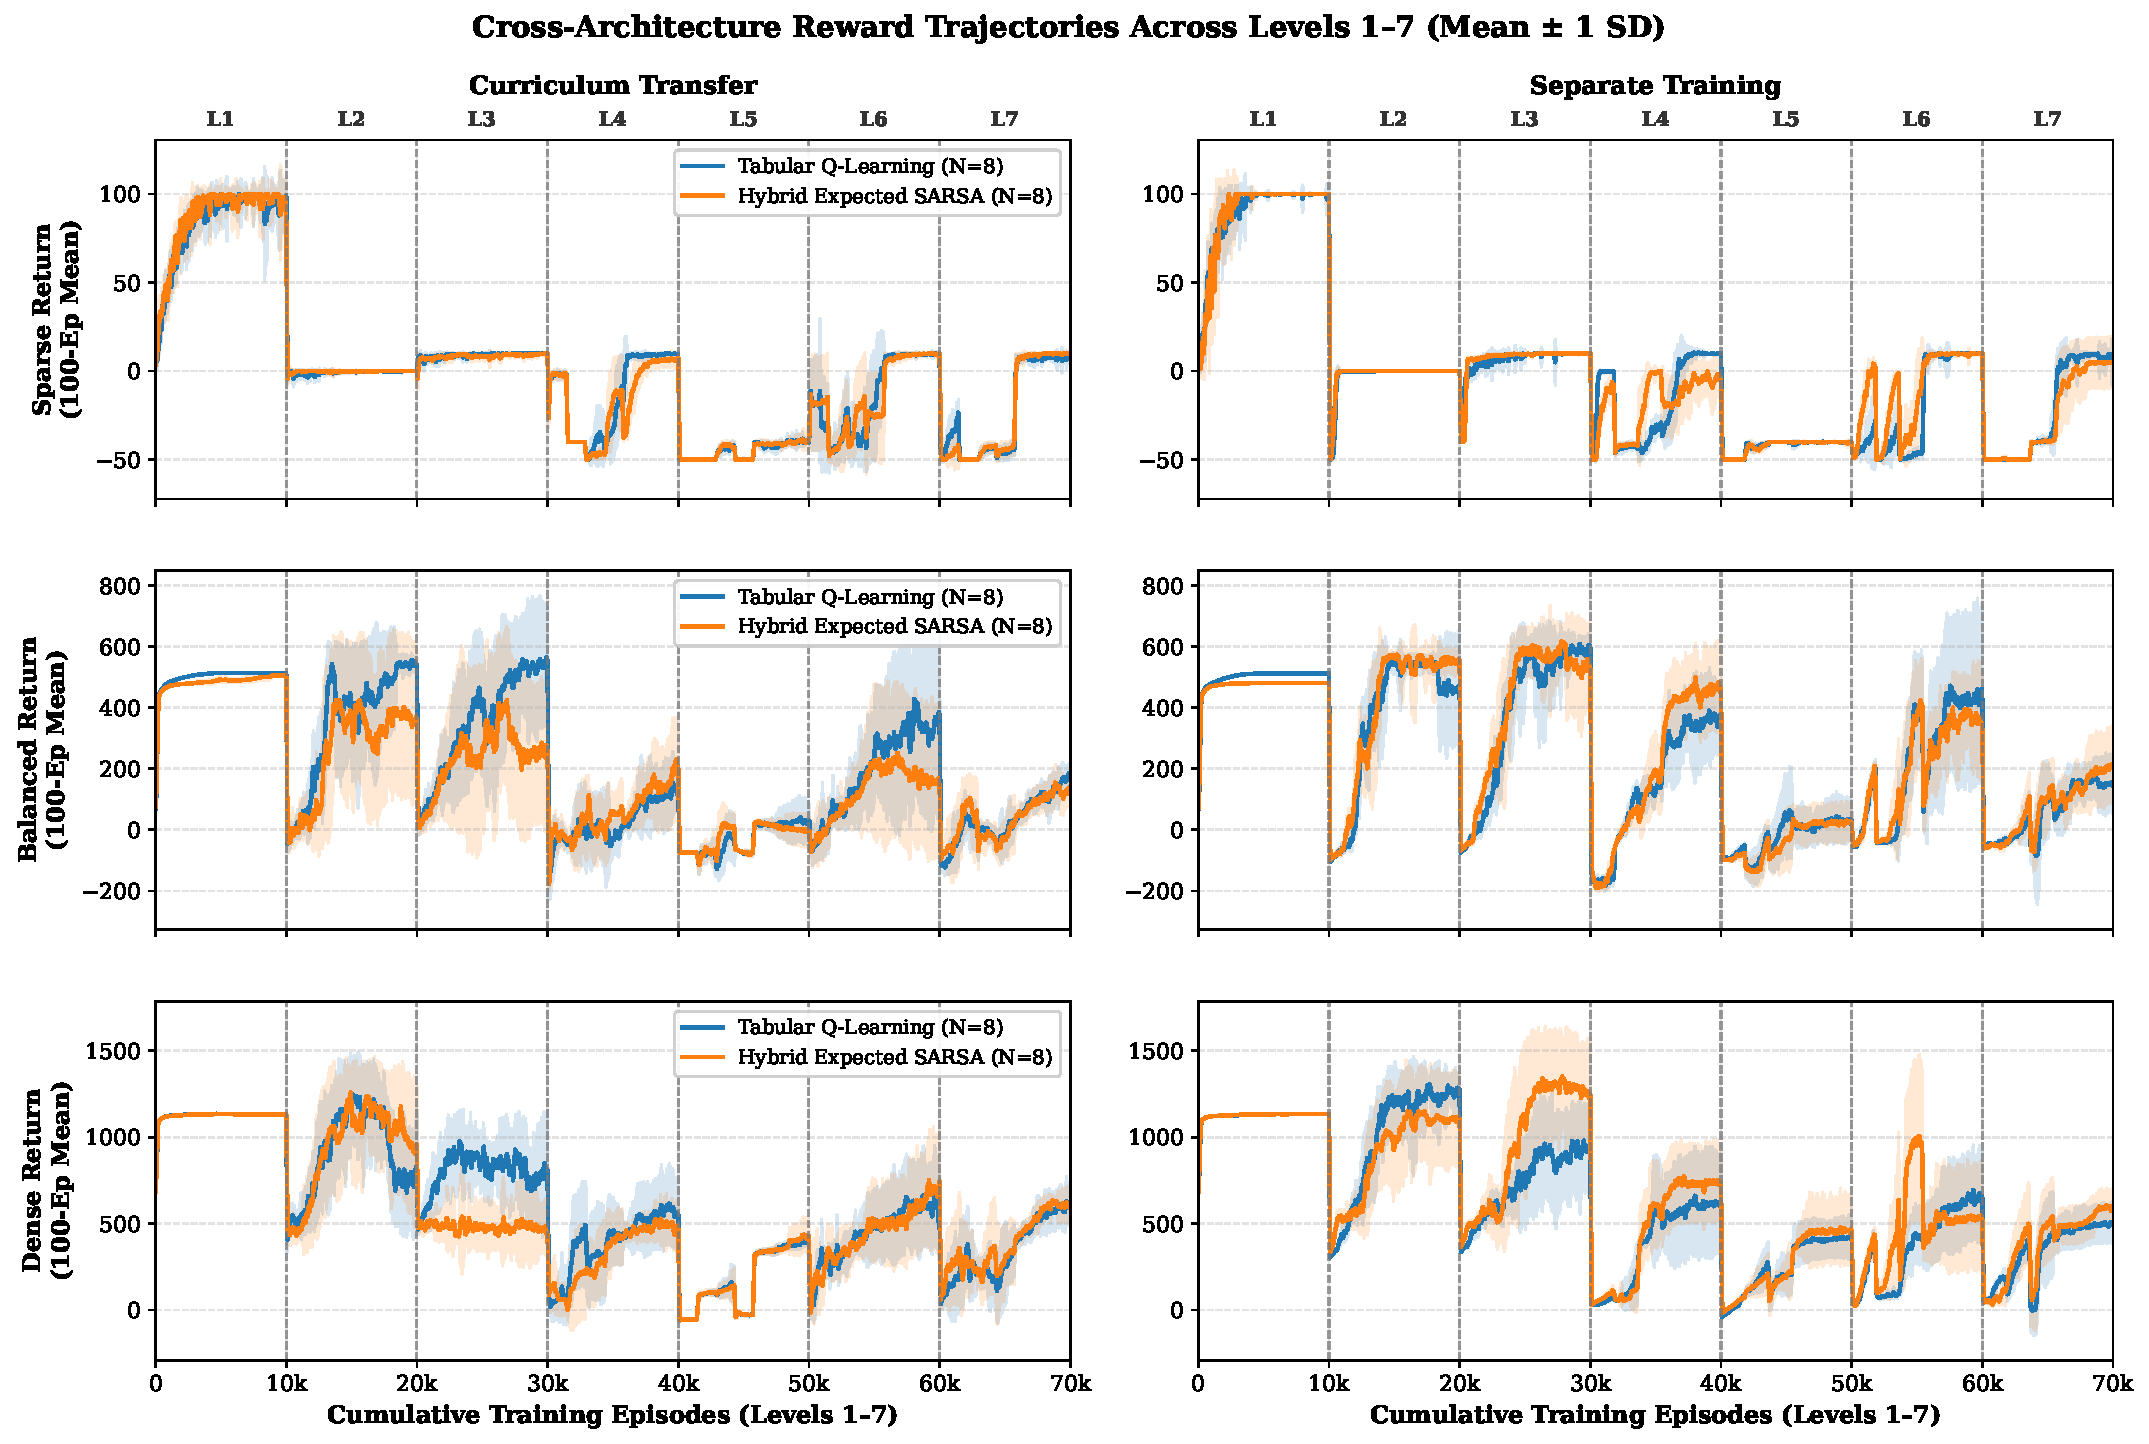
\includegraphics[width=\textwidth]{figures/fig1_reward_trajectories.pdf}
\caption{100-episode rolling reward trajectories (mean $\pm$ 1 SD across 8 seeds) for Sparse (top), Balanced (middle), and Dense (bottom) rewards under Curriculum (left) and Separate (right) training across Levels~1--7.}
\label{fig:reward_trajectories}
\end{figure}

Comparing the three reward settings shows a clear pattern:
\begin{itemize}
    \item \textbf{Sparse fails after Level~1.} On Level~1, agents still reach $87.5\%$--$100.0\%$ Train100 win rates ($50.0\%$--$100.0\%$ Greedy50). From Level~2 to Level~7, every agent and mode ends at $0.0 \pm 0.0\%$. Without step-by-step reward feedback, random exploration rarely finishes a full stage. In Fig.~\ref{fig:reward_trajectories} (top row), Sparse returns on Levels~4--7 briefly rise near $0$--$10$ during reverse-spawn segments close to the goal, but drop back once the spawn shifts to the normal start.
    \item \textbf{Dense encourages rushing and fails on Levels~4--7.} Dense gives $+1.2$ per pixel decrease in goal distance, with a smaller death penalty ($-60.0$) and no hazard-timing penalties. It learns Level~1 ($100.0\%$ Train100) and gets moderate results on Level~2 ($41.8\%$--$86.5\%$ Train100) and Level~3 ($0.0\%$--$60.8\%$), though usually worse than Balanced. On Levels~4--7, Dense gets $0.0\%$ on Levels~4, 5, and 7, and at most $1.5\%$ Train100 ($0.0\%$ Greedy50) on Level~6. Even when Dense shows high return curves in Fig.~\ref{fig:reward_trajectories} (around $+500$ to $+1{,}300$), the agent is only collecting forward-movement points before running into hazards.
    \item \textbf{Balanced is the best reward choice.} Balanced wins $100.0\%$ on Level~1, up to $95.4\%$ Train100 ($100.0\%$ Greedy50) on Level~2, and up to $80.5\%$ Train100 ($100.0\%$ Greedy50) on Level~3. It is also the only reward that wins on Level~4 ($19.6\%$ Train100 / $37.5\%$ Greedy50 for Hybrid Separate) and gets solid wins on Level~6 ($30.8\%$ Train100 / $50.0\%$ Greedy50 for Tabular Separate). For this reason, we keep Reward fixed to \textbf{Balanced} in Sections~\ref{subsec:curr_vs_sep}--\ref{subsec:failures}.
\end{itemize}

\subsection{Curriculum vs.\ Separate \& Agent Comparison}
\label{subsec:curr_vs_sep}

With Reward fixed to \textbf{Balanced}, Fig.~\ref{fig:balanced_overview} shows the full 7-level rolling win-rate curves for both agents and training modes, and Fig.~\ref{fig:spotlight_l3_l4_l6} zooms in on Levels~3, 4, and 6.

\begin{figure}[t]
\centering
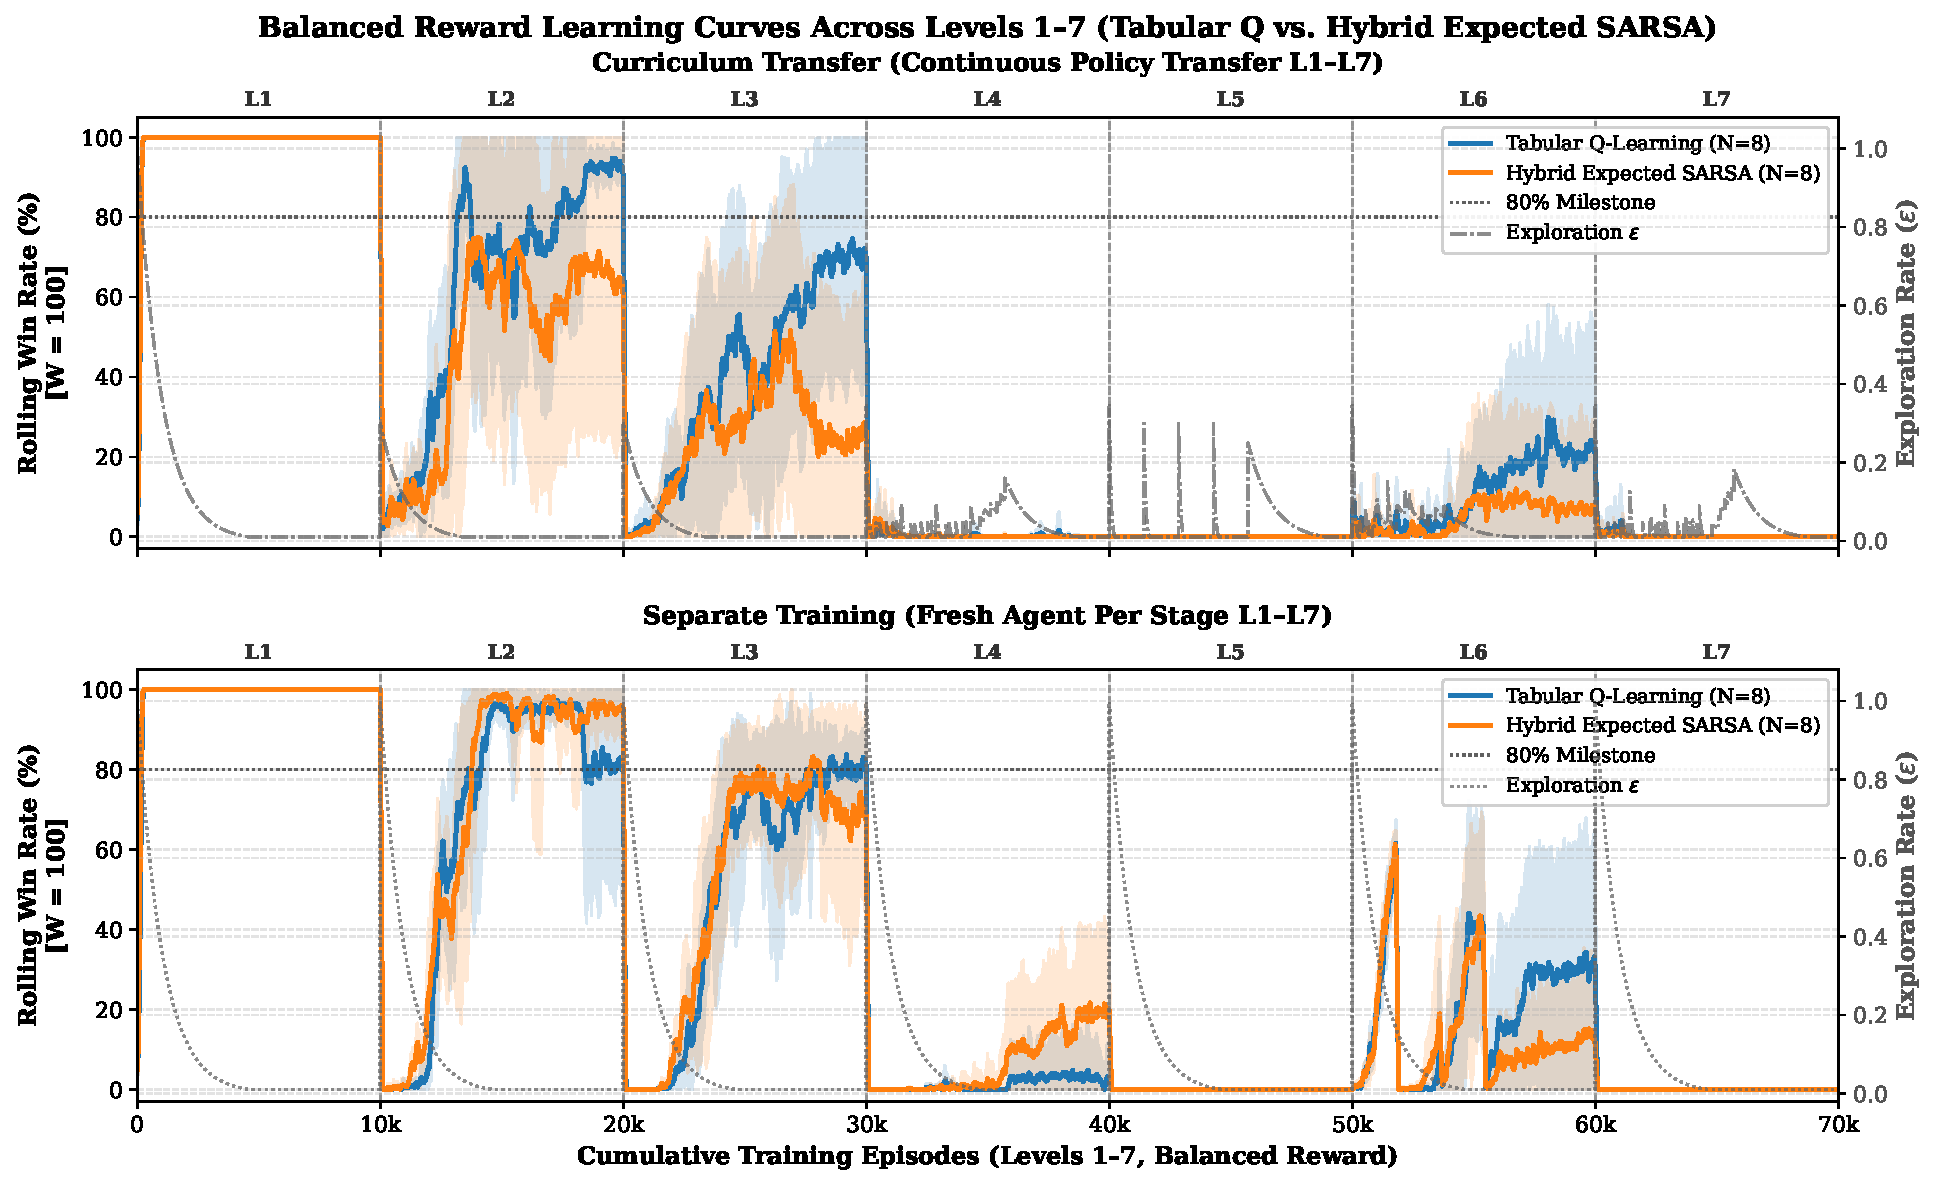
\includegraphics[width=\textwidth]{figures/fig2_balanced_overview.pdf}
\caption{Balanced-reward 100-episode rolling win rate (mean $\pm$ 1 SD) and exploration rate $\epsilon$ across Levels~1--7 for Curriculum Transfer (top) and Separate Training (bottom).}
\label{fig:balanced_overview}
\end{figure}

\begin{figure}[t]
\centering
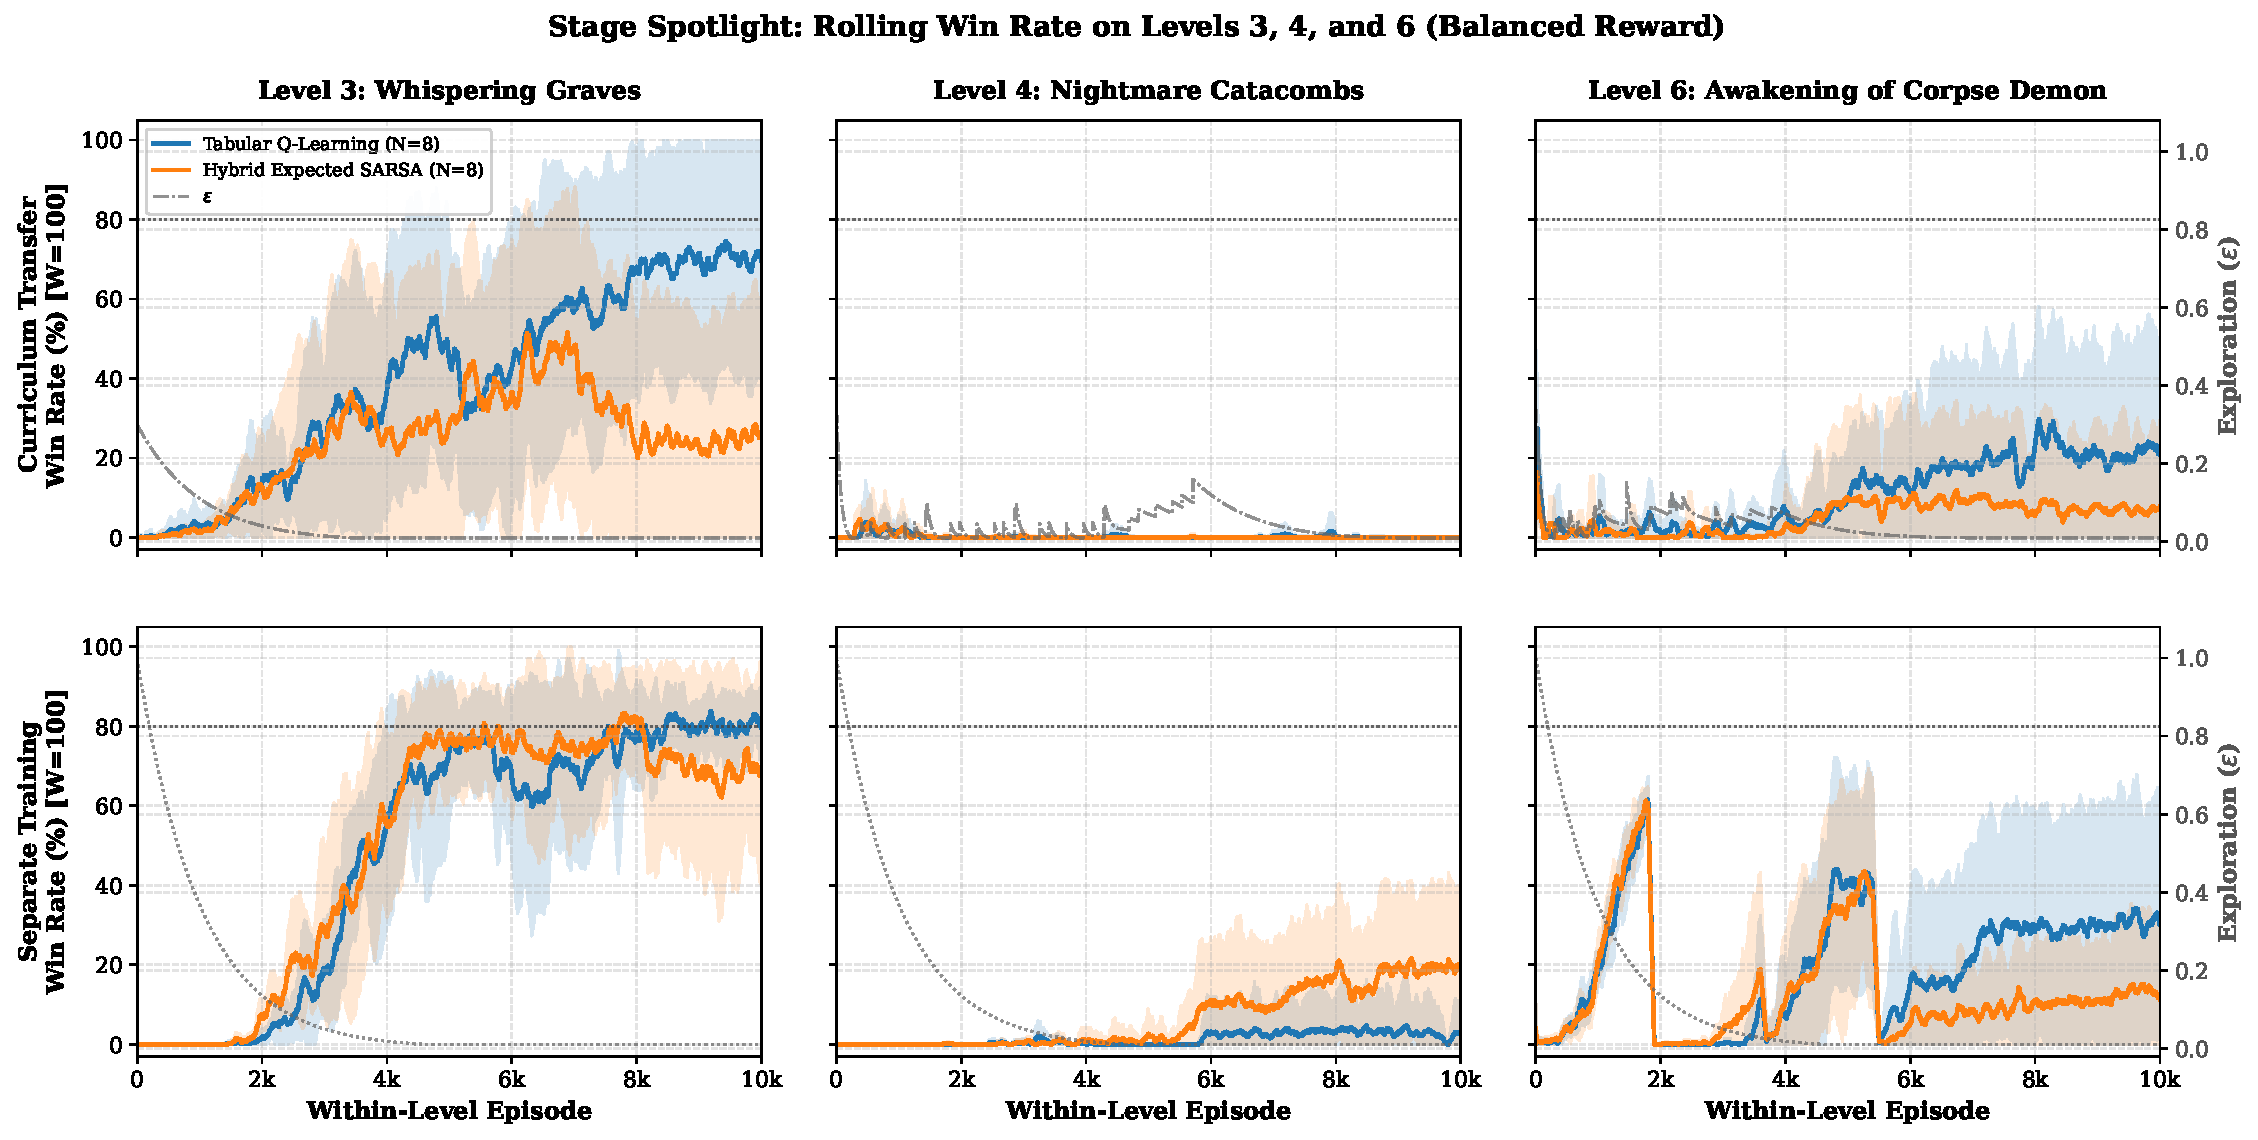
\includegraphics[width=\textwidth]{figures/fig3_spotlight_l3_l4_l6.pdf}
\caption{Within-level rolling win rate on Levels~3, 4, and 6 under Balanced reward for Curriculum Transfer (top) and Separate Training (bottom).}
\label{fig:spotlight_l3_l4_l6}
\end{figure}

Across the two agents, neither wins everywhere. Both reach $100.0 \pm 0.0\%$ on Level~1. On Level~2, Tabular beats Hybrid in Curriculum ($90.8 \pm 5.5\%$ vs.\ $60.6 \pm 41.7\%$ Train100; $100.0\%$ vs.\ $62.5\%$ Greedy50), while Hybrid beats Tabular in Separate ($95.4 \pm 5.4\%$ vs.\ $82.1 \pm 26.9\%$ Train100; $100.0\%$ vs.\ $75.0\%$ Greedy50). On Level~3 and Level~6, Tabular outperforms Hybrid in both modes: on Level~3, Tabular reaches $69.6\%$ (Curriculum) and $80.5\%$ (Separate) vs.\ $26.0\%$ and $67.6\%$ for Hybrid; on Level~6, Tabular reaches $21.2\%$ (Curriculum) and $30.8\%$ (Separate) vs.\ $7.8\%$ and $11.2\%$ for Hybrid. On Level~4, however, Hybrid Separate outperforms Tabular Separate ($19.6 \pm 19.0\%$ vs.\ $2.9 \pm 8.1\%$ Train100; $37.5\%$ vs.\ $12.5\%$ Greedy50) because Expected SARSA lowers the value of states where random exploratory steps near moving hazards can kill the agent.

One surprising result is that \textbf{Separate training beats Curriculum transfer on Levels~3, 4, and 6}:
\begin{itemize}
    \item \textbf{Level~3}: Tabular Separate gets $80.5\%$ Train100 ($100.0\%$ Greedy50) vs.\ $69.6\%$ ($75.0\%$) for Tabular Curriculum; Hybrid Separate gets $67.6\%$ ($87.5\%$) vs.\ $26.0\%$ ($25.0\%$) for Hybrid Curriculum. In Fig.~\ref{fig:spotlight_l3_l4_l6} (left column), Curriculum starts climbing earlier because it already knows basic jumping from Levels~1--2, but Separate starts from $\epsilon = 1.0$, explores more broadly, and settles at a higher win rate with lower variance across seeds.
    \item \textbf{Level~4}: Both Curriculum agents end at $0.0 \pm 0.0\%$, while Separate reaches $19.6\%$ (Hybrid) and $2.9\%$ (Tabular) Train100. In Curriculum mode, $\epsilon$ only re-warms to $0.35$ (and decays quickly at $0.985$ during reverse spawns), while the $50\%$ round-robin replay of Levels~1--3 keeps pulling shared Q-values back toward simpler levels that lack dynamic hazards.
    \item \textbf{Level~6}: Tabular Separate gets $30.8\%$ Train100 ($50.0\%$ Greedy50) vs.\ $21.2\%$ ($25.0\%$) in Curriculum, and Hybrid Separate gets $11.2\%$ vs.\ $7.8\%$ in Curriculum.
\end{itemize}

On Level~6 Separate (Fig.~\ref{fig:spotlight_l3_l4_l6}, bottom right), both agents show two sharp drops around episodes $1{,}800$ ($1.8\text{k}$) and $5{,}400$ ($5.4\text{k}$). This comes directly from the fixed reverse-spawn schedule in \texttt{training/trainer.py}. For episodes $1$--$1{,}800$ ($\le 18\%$ of $10{,}000$), the agent spawns at $0.75$ of the goal distance, so it quickly learns the short final section and reaches about $60\%$ rolling win rate. At episode $1{,}801$, the spawn jumps back to $0.50$ of the goal distance while $\epsilon$ has already decayed to about $0.165$, causing an immediate drop to $0\%$. The agents recover through the $0.50$ and $0.25$ blocks (with a smaller dip around $3.6\text{k}$), climbing above $40\%$ before episode $5{,}400$. At episode $5{,}401$, the spawn switches to the true level start. By then $\epsilon$ has already reached its $0.01$ floor, and because Separate mode does not re-warm $\epsilon$ on spawn shifts, the win rate drops sharply again before slowly recovering to $30.8\%$ (Tabular) and $11.2\%$ (Hybrid).

\subsection{Sample Efficiency}
\label{subsec:sample_efficiency}

Holding Reward fixed to \textbf{Balanced}, Table~\ref{tab:sample_efficiency} and Fig.~\ref{fig:sample_efficiency} compare how fast the agents reach an $80.0\%$ 100-episode rolling win rate and how many simulator steps they spend across Levels~1--7. We separate \textit{Adaptation Steps} (steps inside the current level up to $80\%$ WR), \textit{Pre-Training Steps} (steps spent on earlier levels in Curriculum mode), \textit{Global Steps} (Pre-Training + Adaptation for converging seeds), and \textit{Total Stage Steps} (all steps across the full $10{,}000$-episode stage).

\begin{table}[t]
\caption{Sample efficiency and compute cost (Balanced reward, Levels~1--7). Ep to 80\% WR, Adaptation, Pre-Training, and Global Steps average over the $k/8$ converging seeds; Total Stage Steps averages over all 8 seeds. DNC = Did Not Converge.}
\label{tab:sample_efficiency}
\centering
\resizebox{\textwidth}{!}{%
\begin{tabular}{llcccccc}
\toprule
\textbf{Level} & \textbf{Agent \& Mode} & \textbf{Conv. ($k/N$)} & \textbf{Ep to 80\% WR} & \textbf{Adaptation Steps} & \textbf{Pre-Training Steps} & \textbf{Global Steps to 80\% WR} & \textbf{Total Stage Steps} \\
\midrule
Level 1 & Tabular Curriculum & 8/8 & 165.8 $\pm$ 8.6 & 122,356 $\pm$ 5,963 & 0 $\pm$ 0 & 122,356 $\pm$ 5,963 & 2,050,584 $\pm$ 19,218 \\
Level 1 & Tabular Separate & 8/8 & 176.6 $\pm$ 7.5 & 131,197 $\pm$ 5,302 & 0 & 131,197 $\pm$ 5,302 & 2,163,960 $\pm$ 14,177 \\
Level 1 & Hybrid Expected Curriculum & 8/8 & 160.9 $\pm$ 7.9 & 118,493 $\pm$ 5,660 & 0 $\pm$ 0 & 118,493 $\pm$ 5,660 & 2,348,493 $\pm$ 53,081 \\
Level 1 & Hybrid Expected Separate & 8/8 & 156.5 $\pm$ 8.9 & 115,373 $\pm$ 6,380 & 0 & 115,373 $\pm$ 6,380 & 2,398,197 $\pm$ 3,466 \\
\midrule
Level 2 & Tabular Curriculum & 8/8 & 3,039.9 $\pm$ 284.1 & 630,189 $\pm$ 73,589 & 2,050,584 $\pm$ 19,218 & 2,680,773 $\pm$ 68,334 & 2,383,546 $\pm$ 76,340 \\
Level 2 & Tabular Separate & 8/8 & 3,262.6 $\pm$ 456.8 & 900,836 $\pm$ 137,296 & 0 & 900,836 $\pm$ 137,296 & 2,917,696 $\pm$ 105,929 \\
Level 2 & Hybrid Expected Curriculum & 8/8 & 3,595.8 $\pm$ 1,332.6 & 746,716 $\pm$ 154,209 & 2,348,493 $\pm$ 53,081 & 3,095,208 $\pm$ 167,652 & 2,412,382 $\pm$ 208,318 \\
Level 2 & Hybrid Expected Separate & 8/8 & 3,410.5 $\pm$ 585.3 & 970,581 $\pm$ 190,875 & 0 & 970,581 $\pm$ 190,875 & 2,912,790 $\pm$ 146,503 \\
\midrule
Level 3 & Tabular Curriculum & 7/8 & 5,250.1 $\pm$ 2,246.9 & 1,331,804 $\pm$ 515,862 & 4,431,503 $\pm$ 80,938 & 5,763,307 $\pm$ 540,010 & 2,829,690 $\pm$ 338,387 \\
Level 3 & Tabular Separate & 8/8 & 4,675.1 $\pm$ 917.9 & 1,517,500 $\pm$ 429,207 & 0 & 1,517,500 $\pm$ 429,207 & 3,382,402 $\pm$ 278,286 \\
Level 3 & Hybrid Expected Curriculum & 4/8 & 4,683.5 $\pm$ 2,153.7 & 1,137,576 $\pm$ 369,924 & 4,679,752 $\pm$ 251,585 & 5,817,328 $\pm$ 467,288 & 2,671,212 $\pm$ 387,524 \\
Level 3 & Hybrid Expected Separate & 7/8 & 4,410.0 $\pm$ 807.7 & 1,275,779 $\pm$ 336,151 & 0 & 1,275,779 $\pm$ 336,151 & 3,263,836 $\pm$ 283,039 \\
\midrule
Level 4 & Tabular Curriculum & 0/8 & DNC & DNC & DNC & DNC & 2,688,631 $\pm$ 514,390 \\
Level 4 & Tabular Separate & 0/8 & DNC & DNC & 0 & DNC & 2,533,682 $\pm$ 190,026 \\
Level 4 & Hybrid Expected Curriculum & 0/8 & DNC & DNC & DNC & DNC & 2,157,214 $\pm$ 476,690 \\
Level 4 & Hybrid Expected Separate & 0/8 & DNC & DNC & 0 & DNC & 2,563,432 $\pm$ 221,571 \\
\midrule
Level 5 & Tabular Curriculum & 0/8 & DNC & DNC & DNC & DNC & 822,320 $\pm$ 62,509 \\
Level 5 & Tabular Separate & 0/8 & DNC & DNC & 0 & DNC & 1,084,920 $\pm$ 228,581 \\
Level 5 & Hybrid Expected Curriculum & 0/8 & DNC & DNC & DNC & DNC & 853,636 $\pm$ 82,909 \\
Level 5 & Hybrid Expected Separate & 0/8 & DNC & DNC & 0 & DNC & 909,847 $\pm$ 104,445 \\
\midrule
Level 6 & Tabular Curriculum & 1/8 & 6,388.0 & 1,366,889 & 9,419,566 & 10,786,455 & 2,339,462 $\pm$ 697,104 \\
Level 6 & Tabular Separate & 2/8 & 7,043.0 $\pm$ 3,245.6 & 1,473,665 $\pm$ 1,137,251 & 0 & 1,473,665 $\pm$ 1,137,251 & 2,332,832 $\pm$ 501,266 \\
Level 6 & Hybrid Expected Curriculum & 0/8 & DNC & DNC & DNC & DNC & 2,133,405 $\pm$ 612,632 \\
Level 6 & Hybrid Expected Separate & 0/8 & DNC & DNC & 0 & DNC & 2,143,057 $\pm$ 335,087 \\
\midrule
Level 7 & Tabular Curriculum & 0/8 & DNC & DNC & DNC & DNC & 1,789,969 $\pm$ 150,160 \\
Level 7 & Tabular Separate & 0/8 & DNC & DNC & 0 & DNC & 1,670,050 $\pm$ 332,654 \\
Level 7 & Hybrid Expected Curriculum & 0/8 & DNC & DNC & DNC & DNC & 1,770,178 $\pm$ 152,428 \\
Level 7 & Hybrid Expected Separate & 0/8 & DNC & DNC & 0 & DNC & 1,680,126 $\pm$ 272,547 \\
\bottomrule
\end{tabular}%
}
\end{table}

\begin{figure}[t]
\centering
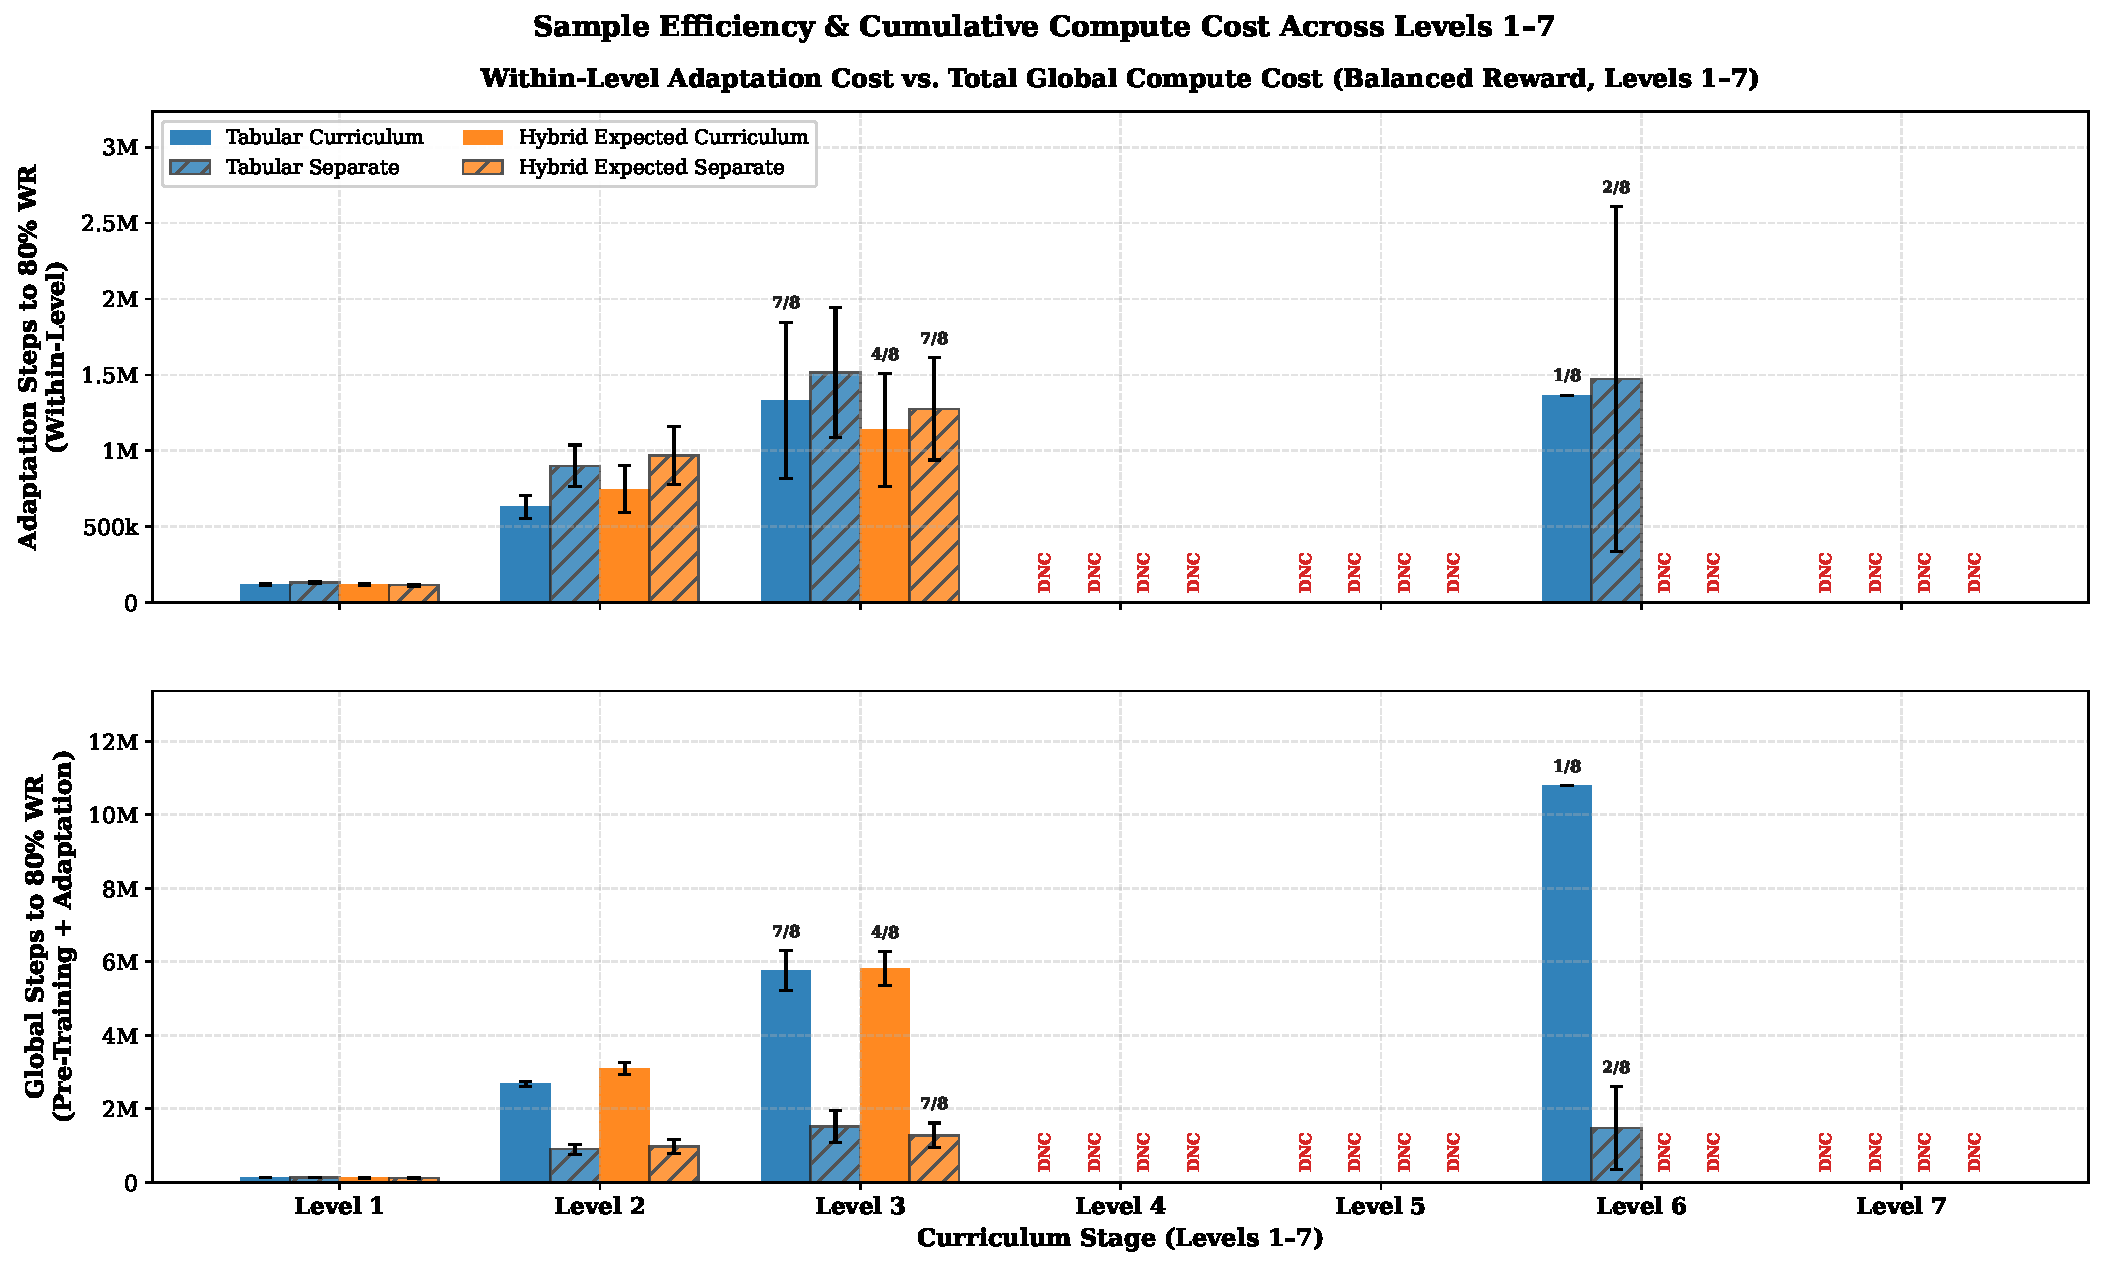
\includegraphics[width=\textwidth]{figures/fig4_sample_efficiency.pdf}
\caption{Within-level adaptation steps (top) and global compute steps (bottom) to reach an $80\%$ rolling win rate under Balanced reward across Levels~1--7.}
\label{fig:sample_efficiency}
\end{figure}

Three points stand out in Table~\ref{tab:sample_efficiency} and Fig.~\ref{fig:sample_efficiency}:
\begin{enumerate}
    \item \textbf{Within-level speed vs.\ global compute.} On Level~1, all four settings converge on $8/8$ seeds in $156.5$--$176.6$ episodes ($115{,}373$--$131{,}197$ steps). On Level~2, all four still converge on $8/8$ seeds, and Curriculum cuts within-level adaptation steps by $30.0\%$ for Tabular ($630{,}189$ vs.\ $900{,}836$) and $23.1\%$ for Hybrid ($746{,}716$ vs.\ $970{,}581$). However, once we add the $2.05\text{M}$--$2.35\text{M}$ pre-training steps from Level~1, Curriculum takes nearly $3\times$ more global steps ($2.68\text{M}$ and $3.10\text{M}$ vs.\ $0.90\text{M}$ and $0.97\text{M}$).
    \item \textbf{Lower convergence rate on Level~3 and Level~6.} On Level~3, Separate reaches $80\%$ WR more reliably ($8/8$ for Tabular, $7/8$ for Hybrid) than Curriculum ($7/8$ for Tabular, $4/8$ for Hybrid), while requiring only $1.28\text{M}$--$1.52\text{M}$ global steps compared to $5.76\text{M}$--$5.82\text{M}$ for Curriculum. On Level~6, only Tabular converges on a few seeds ($2/8$ Separate at $1.47\text{M}$ steps; $1/8$ Curriculum at $10.79\text{M}$ global steps), while Hybrid stays at $0/8$.
    \item \textbf{Total stage steps reflect survival time.} Levels~4, 5, and 7 never hit $80\%$ WR ($0/8$ DNC). Level~5 has the lowest Total Stage Steps ($0.82\text{M}$--$1.08\text{M}$, around $82$--$108$ steps per episode) because agents die early in pits and hazards, whereas Level~1 spends $2.05\text{M}$--$2.40\text{M}$ steps across $10{,}000$ full winning runs.
\end{enumerate}

\subsection{Why Hard Levels Fail \& Limitations}
\label{subsec:failures}

Table~\ref{tab:failure_modes} summarizes the outcome breakdown and discovered state counts on Levels~4--7 under Balanced reward. Note that unlike Table~\ref{tab:overall_winrates} (which reports only the final 100 episodes), the Win \%, Timeout \%, Pit Death \%, and Hazard/Entity Death \% columns in Table~\ref{tab:failure_modes} are averaged across \textbf{all $10{,}000$ training episodes} per stage (including early reverse-spawn episodes). Hazard/Entity Death \% groups all non-pit lethal collisions (ghosts, fire, lasers, wisps, and grave monsters).

\begin{table}[t]
\caption{Failure breakdown and discovered state counts on Levels~4--7 (Balanced reward). Percentages average across all $10{,}000$ training episodes per level across 8 seeds.}
\label{tab:failure_modes}
\centering
\resizebox{\textwidth}{!}{%
\begin{tabular}{llccccc}
\toprule
\textbf{Level} & \textbf{Agent \& Mode} & \textbf{Win \% (All 10k)} & \textbf{Timeout \%} & \textbf{Pit Death \%} & \textbf{Hazard/Entity Death \%} & \textbf{Discovered States} \\
\midrule
Level 4 & Tabular Curriculum & 0.2 $\pm$ 0.2\% & 42.0 $\pm$ 7.2\% & 36.8 $\pm$ 7.1\% & 20.9 $\pm$ 3.5\% & 1,672 $\pm$ 187 \\
Level 4 & Tabular Separate & 1.3 $\pm$ 3.3\% & 52.4 $\pm$ 4.2\% & 25.6 $\pm$ 2.0\% & 20.7 $\pm$ 2.7\% & 1,562 $\pm$ 57 \\
Level 4 & Hybrid Expected Curriculum & 0.2 $\pm$ 0.2\% & 38.7 $\pm$ 7.6\% & 38.7 $\pm$ 10.4\% & 22.4 $\pm$ 5.0\% & 1,690 $\pm$ 103 \\
Level 4 & Hybrid Expected Separate & 6.6 $\pm$ 6.3\% & 47.1 $\pm$ 11.6\% & 19.1 $\pm$ 3.0\% & 27.3 $\pm$ 8.4\% & 1,771 $\pm$ 66 \\
\midrule
Level 5 & Tabular Curriculum & 0.0 $\pm$ 0.0\% & 40.1 $\pm$ 5.3\% & 26.3 $\pm$ 4.9\% & 33.6 $\pm$ 5.9\% & 5,688 $\pm$ 343 \\
Level 5 & Tabular Separate & 0.0 $\pm$ 0.0\% & 26.1 $\pm$ 6.0\% & 46.6 $\pm$ 10.9\% & 27.2 $\pm$ 6.0\% & 4,616 $\pm$ 392 \\
Level 5 & Hybrid Expected Curriculum & 0.0 $\pm$ 0.0\% & 43.2 $\pm$ 5.8\% & 31.8 $\pm$ 6.0\% & 24.9 $\pm$ 6.0\% & 5,718 $\pm$ 188 \\
Level 5 & Hybrid Expected Separate & 0.0 $\pm$ 0.0\% & 22.1 $\pm$ 3.6\% & 48.6 $\pm$ 12.9\% & 29.3 $\pm$ 12.0\% & 4,358 $\pm$ 337 \\
\midrule
Level 6 & Tabular Curriculum & 10.9 $\pm$ 10.8\% & 33.7 $\pm$ 5.0\% & 15.9 $\pm$ 8.2\% & 39.5 $\pm$ 10.3\% & 6,716 $\pm$ 257 \\
Level 6 & Tabular Separate & 19.6 $\pm$ 13.0\% & 33.3 $\pm$ 10.7\% & 8.5 $\pm$ 6.6\% & 38.5 $\pm$ 7.1\% & 2,077 $\pm$ 125 \\
Level 6 & Hybrid Expected Curriculum & 5.0 $\pm$ 11.2\% & 38.0 $\pm$ 5.9\% & 27.7 $\pm$ 14.8\% & 29.2 $\pm$ 9.2\% & 6,726 $\pm$ 186 \\
Level 6 & Hybrid Expected Separate & 13.3 $\pm$ 7.8\% & 33.8 $\pm$ 11.1\% & 12.2 $\pm$ 6.4\% & 40.7 $\pm$ 7.5\% & 1,973 $\pm$ 70 \\
\midrule
Level 7 & Tabular Curriculum & 0.2 $\pm$ 0.3\% & 49.9 $\pm$ 5.6\% & 23.2 $\pm$ 4.5\% & 26.7 $\pm$ 4.5\% & 9,413 $\pm$ 302 \\
Level 7 & Tabular Separate & 0.0 $\pm$ 0.0\% & 53.0 $\pm$ 5.6\% & 26.3 $\pm$ 5.8\% & 20.7 $\pm$ 3.4\% & 4,326 $\pm$ 419 \\
Level 7 & Hybrid Expected Curriculum & 0.1 $\pm$ 0.1\% & 41.5 $\pm$ 6.6\% & 29.2 $\pm$ 6.6\% & 29.1 $\pm$ 4.3\% & 9,130 $\pm$ 194 \\
Level 7 & Hybrid Expected Separate & 0.0 $\pm$ 0.0\% & 50.5 $\pm$ 7.2\% & 28.5 $\pm$ 6.4\% & 20.9 $\pm$ 3.9\% & 4,187 $\pm$ 365 \\
\bottomrule
\end{tabular}%
}
\end{table}

Table~\ref{tab:failure_modes} shows clear failure patterns across the hard stages:
\begin{itemize}
    \item \textbf{Level~4 (Timeouts and pits):} Timeouts are the largest share ($38.7\%$--$52.4\%$), followed by pit deaths ($19.1\%$--$38.7\%$) and hazard deaths ($20.7\%$--$27.3\%$). Separate training cuts pit deaths down to $19.1\%$ (Hybrid) and $25.6\%$ (Tabular), but many runs still stall until timeout in front of moving hazards.
    \item \textbf{Level~5 ($0.0\%$ wins across all 10k episodes):} Separate agents die mostly in pits ($46.6\%$ Tabular, $48.6\%$ Hybrid) and hazards ($27.2\%$--$29.3\%$), while Curriculum agents stall more often ($40.1\%$--$43.2\%$ timeouts).
    \item \textbf{Level~6 (Partial wins, mostly hazard deaths):} Hazard/entity deaths are the main failure ($29.2\%$--$40.7\%$) alongside timeouts ($33.3\%$--$38.0\%$), whereas pit deaths drop to $8.5\%$--$12.2\%$ in Separate mode.
    \item \textbf{Level~7 (Timeouts dominate):} Timeouts account for $41.5\%$--$53.0\%$ of episodes, with $23.2\%$--$29.2\%$ pit deaths and $20.7\%$--$29.1\%$ hazard deaths, leaving near-zero wins ($0.0\%$--$0.2\%$).
\end{itemize}

Four main limitations explain why these failures happen:
\begin{enumerate}
    \item \textbf{15-tuple state space and perceptual aliasing:} In \texttt{discretizer/state\_discretizer.py}, continuous game states are quantized into a 15-tuple (\texttt{grounded}, \texttt{vy}, \texttt{obs\_dist}, \texttt{obs\_height}, \texttt{pit\_dist}, \texttt{ghost\_dist}, \texttt{ghost\_alt}, \texttt{laser}, \texttt{wisp}, \texttt{crouch}, \texttt{double\_jump}, \texttt{monster}, \texttt{pit\_width}, \texttt{ghost\_vx}, \texttt{vx}) with $8{,}847{,}360$ theoretical states. In practice, agents only visit $1{,}562$--$9{,}413$ states (under $0.11\%$). Because each bin tracks only the nearest entity within coarse distance ranges (such as $0$--$80\text{ px}$ or $0$--$100\text{ px}$) without exact timers or multi-entity ordering, different hazard combinations fall into the same discrete state. A tabular Q-table averages those conflicting outcomes, leading either to hesitation (timeouts) or mistimed jumps (pit and hazard deaths).
    \item \textbf{Negative transfer in Curriculum mode:} Curriculum carries Q-values from earlier stages and replays prior levels on $50\%$ of episodes. Look at Table~\ref{tab:failure_modes}: on Level~6, Curriculum uses $6{,}716$--$6{,}726$ cumulative states, while Separate reaches higher win rates using only $1{,}973$--$2{,}077$ states. Replaying simpler stages pulls shared aliased states back toward habits that fail under combined hazards.
    \item \textbf{Exploration schedule on reverse spawns:} In Separate mode, $\epsilon$ decays to $0.01$ around episode $4{,}603$, before the full-level phase starts at episode $5{,}401$, leaving too little exploration for the start of Levels~5--7.
    \item \textbf{Fixed bin thresholds:} Distance and velocity cutoffs are tuned by hand, so changing level timing or adding simultaneous enemies cannot be fixed without a richer model such as a neural network.
\end{enumerate}

\subsection{Checkpoint Blind Evaluation (1,000 Procedural Episodes per Level)}
\label{subsec:checkpoint_eval}

To test how well the trained policies work on unseen layouts, we take each saved best per-level checkpoint (\texttt{q\_table\_lvl\{1..7\}\_best.pkl}) and run a blind greedy test ($\epsilon = 0.0$) over $1{,}000$ procedural maps generated by \texttt{LevelGenerator} (map seeds $1$--$1{,}000$) in \texttt{evaluation/eval\_checkpoints\_1000.py}. Table~\ref{tab:checkpoint_blind} reports the mean $\pm$ SD win rate and episode reward across the $8$ training seeds ($42$--$49$) for all $7$ levels, $2$ agents, $2$ modes, and $3$ rewards.

\begin{table}[t]
\caption{Blind greedy evaluation over $1{,}000$ procedural map seeds per level (mean $\pm$ SD across 8 training seeds). Values show Win Rate (\%) / Mean Episode Reward.}
\label{tab:checkpoint_blind}
\centering
\resizebox{\textwidth}{!}{%
\begin{tabular}{llcccc}
\toprule
\textbf{Level} & \textbf{Reward} & \textbf{Tabular Curr} & \textbf{Hybrid Curr} & \textbf{Tabular Sep} & \textbf{Hybrid Sep} \\
 & & \textbf{(WR \% / Reward)} & \textbf{(WR \% / Reward)} & \textbf{(WR \% / Reward)} & \textbf{(WR \% / Reward)} \\
\midrule
Level 1 & Balanced & 97.1 $\pm$ 8.1\% / 696.2 $\pm$ 100.7 & 100.0 $\pm$ 0.0\% / 722.3 $\pm$ 5.0 & 100.0 $\pm$ 0.0\% / 728.5 $\pm$ 3.1 & 98.7 $\pm$ 3.7\% / 670.8 $\pm$ 126.5 \\
Level 1 & Dense & 93.1 $\pm$ 19.4\% / 1,771.2 $\pm$ 196.3 & 100.0 $\pm$ 0.0\% / 1,841.5 $\pm$ 1.5 & 90.1 $\pm$ 23.1\% / 1,749.6 $\pm$ 208.6 & 95.7 $\pm$ 12.1\% / 1,745.6 $\pm$ 261.0 \\
Level 1 & Sparse & 100.0 $\pm$ 0.1\% / 100.0 $\pm$ 0.1 & 90.4 $\pm$ 27.0\% / 90.4 $\pm$ 27.0 & 78.2 $\pm$ 37.3\% / 78.2 $\pm$ 37.3 & 66.0 $\pm$ 38.4\% / 66.0 $\pm$ 38.4 \\
\midrule
Level 2 & Balanced & 1.4 $\pm$ 0.7\% / -316.8 $\pm$ 954.1 & 1.5 $\pm$ 1.6\% / -174.5 $\pm$ 401.9 & 1.7 $\pm$ 1.5\% / 13.0 $\pm$ 55.1 & 3.1 $\pm$ 1.2\% / 45.4 $\pm$ 19.8 \\
Level 2 & Dense & 1.6 $\pm$ 1.2\% / 570.5 $\pm$ 146.0 & 1.1 $\pm$ 1.2\% / 571.1 $\pm$ 89.6 & 1.5 $\pm$ 0.9\% / 618.4 $\pm$ 46.1 & 1.4 $\pm$ 0.6\% / 598.8 $\pm$ 51.6 \\
Level 2 & Sparse & 0.0 $\pm$ 0.0\% / -29.7 $\pm$ 17.2 & 0.0 $\pm$ 0.0\% / -32.6 $\pm$ 13.8 & 0.0 $\pm$ 0.0\% / -44.9 $\pm$ 0.5 & 0.0 $\pm$ 0.0\% / -0.6 $\pm$ 1.7 \\
\midrule
Level 3 & Balanced & 1.7 $\pm$ 1.6\% / 82.2 $\pm$ 52.6 & 2.2 $\pm$ 3.1\% / 75.0 $\pm$ 97.4 & 0.5 $\pm$ 0.2\% / -28.7 $\pm$ 57.5 & 0.8 $\pm$ 0.2\% / 22.0 $\pm$ 4.9 \\
Level 3 & Dense & 0.8 $\pm$ 0.9\% / 596.5 $\pm$ 72.6 & 0.5 $\pm$ 0.8\% / 561.5 $\pm$ 81.1 & 0.1 $\pm$ 0.2\% / 405.8 $\pm$ 42.3 & 0.2 $\pm$ 0.2\% / 442.3 $\pm$ 36.2 \\
Level 3 & Sparse & 0.0 $\pm$ 0.0\% / -29.3 $\pm$ 17.0 & 0.0 $\pm$ 0.0\% / -38.3 $\pm$ 11.0 & 0.0 $\pm$ 0.0\% / -44.3 $\pm$ 0.4 & 0.0 $\pm$ 0.0\% / -41.8 $\pm$ 5.7 \\
\midrule
Level 4 & Balanced & 0.2 $\pm$ 0.2\% / 70.7 $\pm$ 112.9 & 0.3 $\pm$ 0.3\% / 66.8 $\pm$ 121.7 & 0.6 $\pm$ 0.4\% / 142.8 $\pm$ 29.4 & 0.5 $\pm$ 0.4\% / 139.2 $\pm$ 55.6 \\
Level 4 & Dense & 0.1 $\pm$ 0.1\% / 517.0 $\pm$ 70.6 & 0.0 $\pm$ 0.0\% / 496.5 $\pm$ 87.2 & 0.0 $\pm$ 0.0\% / 513.4 $\pm$ 93.1 & 0.0 $\pm$ 0.0\% / 506.1 $\pm$ 38.6 \\
Level 4 & Sparse & 0.0 $\pm$ 0.0\% / -4.4 $\pm$ 5.5 & 0.0 $\pm$ 0.0\% / -5.8 $\pm$ 6.4 & 0.0 $\pm$ 0.0\% / -12.7 $\pm$ 9.9 & 0.0 $\pm$ 0.0\% / -4.4 $\pm$ 9.6 \\
\midrule
Level 5 & Balanced & 0.0 $\pm$ 0.0\% / -8.1 $\pm$ 93.8 & 0.0 $\pm$ 0.0\% / 27.5 $\pm$ 6.6 & 0.0 $\pm$ 0.0\% / 39.2 $\pm$ 8.4 & 0.0 $\pm$ 0.0\% / 27.3 $\pm$ 13.4 \\
Level 5 & Dense & 0.0 $\pm$ 0.0\% / 391.1 $\pm$ 17.4 & 0.0 $\pm$ 0.0\% / 401.5 $\pm$ 15.3 & 0.0 $\pm$ 0.0\% / 410.1 $\pm$ 13.0 & 0.0 $\pm$ 0.0\% / 424.1 $\pm$ 26.6 \\
Level 5 & Sparse & 0.0 $\pm$ 0.0\% / -36.7 $\pm$ 13.2 & 0.0 $\pm$ 0.0\% / -43.0 $\pm$ 1.2 & 0.0 $\pm$ 0.0\% / -36.9 $\pm$ 15.6 & 0.0 $\pm$ 0.0\% / -44.3 $\pm$ 0.2 \\
\midrule
Level 6 & Balanced & 0.5 $\pm$ 0.4\% / 70.6 $\pm$ 23.8 & 0.7 $\pm$ 0.6\% / 92.8 $\pm$ 12.8 & 0.1 $\pm$ 0.1\% / 14.8 $\pm$ 17.4 & 0.1 $\pm$ 0.1\% / 18.5 $\pm$ 21.0 \\
Level 6 & Dense & 0.1 $\pm$ 0.2\% / 427.3 $\pm$ 40.2 & 0.0 $\pm$ 0.1\% / 420.5 $\pm$ 25.8 & 0.0 $\pm$ 0.0\% / 358.1 $\pm$ 34.7 & 0.0 $\pm$ 0.0\% / 352.8 $\pm$ 19.5 \\
Level 6 & Sparse & 0.0 $\pm$ 0.0\% / -28.6 $\pm$ 9.6 & 0.0 $\pm$ 0.0\% / -33.6 $\pm$ 6.5 & 0.0 $\pm$ 0.0\% / -35.5 $\pm$ 9.5 & 0.0 $\pm$ 0.0\% / -25.5 $\pm$ 10.3 \\
\midrule
Level 7 & Balanced & 0.0 $\pm$ 0.0\% / 21.3 $\pm$ 66.2 & 0.0 $\pm$ 0.0\% / 47.5 $\pm$ 14.7 & 0.0 $\pm$ 0.0\% / -11.1 $\pm$ 25.2 & 0.0 $\pm$ 0.0\% / 1.4 $\pm$ 27.1 \\
Level 7 & Dense & 0.0 $\pm$ 0.0\% / 359.7 $\pm$ 49.1 & 0.0 $\pm$ 0.0\% / 388.4 $\pm$ 25.7 & 0.0 $\pm$ 0.0\% / 296.0 $\pm$ 37.3 & 0.0 $\pm$ 0.0\% / 300.5 $\pm$ 33.6 \\
Level 7 & Sparse & 0.0 $\pm$ 0.0\% / -34.7 $\pm$ 7.7 & 0.0 $\pm$ 0.0\% / -42.7 $\pm$ 6.7 & 0.0 $\pm$ 0.0\% / -37.8 $\pm$ 11.0 & 0.0 $\pm$ 0.0\% / -34.0 $\pm$ 9.3 \\
\bottomrule
\end{tabular}%
}
\end{table}

Table~\ref{tab:checkpoint_blind} shows a sharp split between Level~1 and Levels~2--7:
\begin{itemize}
    \item \textbf{Level~1 transfers well to new maps ($66.0\%$--$100.0\%$).} Balanced achieves $97.1\%$--$100.0\%$ and Dense reaches $90.1\%$--$100.0\%$, while Sparse gets $66.0\%$--$100.0\%$. Comparing \texttt{env/map\_levels.py} and \texttt{env/level\_generator.py} explains why: both the fixed and procedural Level~1 maps have only static tombstones on flat ground, with no pits or moving hazards. Because the discretizer tracks local obstacle distance and height relative to the player, the jump timing learned on the fixed map works across procedural Level~1 maps ($1{,}300$--$1{,}700\text{ px}$ long, tombstone heights $36$--$58\text{ px}$). Sparse Separate drops on some seeds ($66.0\%$--$78.2\%$) only because weaker training feedback leaves more ties in the Q-table, causing stalls until timeout.
    \item \textbf{Levels~2--7 drop to $0.0\%$--$3.1\%$ on procedural maps.} Even agents that scored $80\%$--$100\%$ on the fixed training maps (such as Level~2 Balanced at $82.1\%$--$95.4\%$ Train100 and Level~3 Balanced at $67.6\%$--$80.5\%$ in Separate mode) fall to $1.4\%$--$3.1\%$ on procedural Level~2 and $0.5\%$--$2.2\%$ on procedural Level~3. On Levels~4--7, win rates sit between $0.0\%$ and $0.7\%$. There are two clear reasons in the code. First, all training runs used \texttt{map\_seed=None} and \texttt{map\_seed\_interval=0}, so each agent only practiced on one fixed layout per level and overfitted to its exact rhythm. Second, \texttt{LevelGenerator} introduces geometry and hazards that differ from the fixed training maps: on Level~2, the fixed map has only two plain pits without fire ($1{,}100\text{ px}$ long), whereas procedural Level~2 adds fire jets to every pit, puts tombstones right before pits, and stretches the map to $1{,}700$--$2{,}200\text{ px}$. In the raw test logs (\texttt{evaluation/checkpoint\_eval\_1000\_raw.csv}), Level~2 Balanced and Dense runs already suffer $40.6\%$--$69.5\%$ pit deaths and end early at $170.4$--$494.3$ steps on average across the 8 agent/mode/reward settings (out of $1{,}600$ max steps), showing that agents fall quickly when pit timing changes.
    \item \textbf{Dense shows high positive rewards even at $0.0\%$ win rate.} Across Levels~2--7, Dense gets mean rewards between $+296.0$ and $+618.4$ despite winning $0.0\%$--$1.6\%$ of the time. This happens because Dense pays $+1.2$ per pixel moved toward the goal while only charging $-60.0$ for dying. On long procedural maps ($1{,}650$--$3{,}200\text{ px}$), running forward for a few hundred pixels before dying still leaves a large positive score. Balanced penalizes pit deaths by $-200.0$ and pays less per pixel ($+0.4$), so failed runs stay near zero or negative (such as $-316.8$ on Level~2 Tabular Curriculum). Overall, the 1,000-episode test shows that training on a single fixed map is not enough for new procedural levels, especially once pits and moving hazards appear.
\end{itemize}



% Section 8: Conclusion and Future Work (Lead: Member 1, 2, 3, 4)
\section{Conclusion and Future Work}
\label{sec:conclusion}

This paper presented an empirical evaluation and statistical verification of tabular reinforcement learning agents navigating continuous 2D platformer environments. By mapping continuous physics into an invariant 7-tuple discrete representation and combining it with asymmetric progress shaping, our system overcame credit assignment bottlenecks without deep neural networks. Through a comprehensive 5-tier curriculum benchmark across 60,000 simulated episodes, we demonstrated that curriculum transfer is essential for multi-hazard domains: while scratch training failed completely on the Level~5 gauntlet (0.0\% win rate), curriculum transfer enabled effective policy acquisition.

Crucially, our comparative benchmark between off-policy Tabular Q-Learning and Hybrid Expected Q-SARSA revealed a fundamental theoretical boundary: on static obstacle stages, pure Q-learning converges reliably; however, in dynamic adversary domains (Level~4), pure Q-learning experiences catastrophic maximization bias under exploratory jitter (3.0\% win rate). By incorporating the behavior policy expectation directly into the TD bootstrap target, Hybrid Expected Q-SARSA effectively prices in exploration risks near hazard boundaries, achieving a \textbf{98.0\% win rate} with zero adversary collisions ($t(181.9) = 28.45, p < 0.0001$, Cohen's $d = 4.02$). Two-sample Welch's $t$-tests confirmed that curriculum policy transfer and expectation-based bootstrapping deliver statistically superior returns and significant simulation compute savings.

\subsection{Team Reflections and Collaborative Takeaways}
Developing this project across a four-member engineering team yielded several key pedagogical insights:
\begin{itemize}
    \item \textbf{Decoupled Architectural Interfaces}: Establishing strict abstract base contracts in \texttt{core/interfaces.py} at project inception allowed Member~1 (Physics), Member~2 (Agent), Member~3 (Training), and Member~4 (Evaluation) to implement, test, and refactor their respective subsystems independently without merge friction.
    \item \textbf{Value of Early Empirical Telemetry}: Implementing automated logging pipelines early in the development lifecycle enabled rapid diagnostic feedback, exposing reward hacking vulnerabilities in dense shaping, maximization bias in pure Q-learning, and perceptual aliasing in compound hazards before master production training.
\end{itemize}

\subsection{Future Scope and Research Directions}
While tabular and hybrid reinforcement learning provides transparency and sample efficiency within structured state manifolds, several promising research avenues remain:
\begin{enumerate}
    \item \textbf{Continuous Function Approximation and Tile Coding}: Transitioning to Tile Coding, Radial Basis Functions (RBFs), or Deep Q-Networks (DQN) would enable the agent to navigate continuous adversary velocities, non-stationary terrain, and procedurally generated layouts without manual bin tuning.
    \item \textbf{Mitigating Perceptual Aliasing in Compound Hazards}: Integrating multi-entity lookahead sensors or recurrent state memory would resolve spatial occlusions when tall obstacles directly abut open chasms or high/low ghost patrols.
    \item \textbf{Multi-Objective Reward Tuning}: Investigating Pareto-optimal trade-offs between safety margins, speed-running traversal time, and optional item collection could uncover diverse navigation personalities.
\end{enumerate}


% =========================================================================
% REFERENCES (Springer LNCS Style)
% =========================================================================
\bibliographystyle{splncs04}
\bibliography{references}

\end{document}
